\documentclass[11pt,a4paper,spanish]{book}
\usepackage{unir}

%---------------------------
% Rellenar con la información apropiada al trabajo.
%---------------------------
\title{Tensor networks en 
\newline 
algoritmos cuánticos 
\newline
variacionales}
\titulacion{Máster en Computación Cuántica}
\author{Andrés Navas Cáliz}
\date{Julio, 2024}
\director{Dr. Francisco Costa Cano, UNIR}
\codirector{Dr. Arnau Riera Graells, Qilimanjaro Quantum Tech}
\nombreciudad{Murcia, Murcia}

\begin{document}

\maketitle

\frontmatter
\tableofcontents
\listoffigures
%\listoftables

\chapter{Resumen}

La optimización de problemas, en particular la optimización de problemas NP-Duros, es un campo de estudio de gran interés. Algunos de los problemas presentes en este campo, son centrales dentro de la actividad de muchas empresas, organismos e instituciones. \\

Este trabajo se centra en la resolución de problemas NP-Duros utilizando la combinación de dos paradigmas de computación, la computación cuántica y tensor networks. El planteamiento de combinar dos paradigmas de computación diferentes tiene como objetivo mejorar y mitigar las deficiencias que, en la actualidad, posee la computación cuántica. Por un lado, tensor networks es una forma de computación que se basa en operaciones y algoritmos eficientes que se ejecutan en plataformas clásicas, las cuales poseen una gran madurez tecnológica. Por otro lado, la computación cuántica es un paradigma de computación que emplea operaciones, algoritmos y protocolos novedosos, que se ejecutan en plataformas cuánticas, las cuales en la actualidad, se encuentran en un estado de poca madurez tecnológica. \\

En este documento se realiza un estudio de las técnicas de pre-optimización existentes, en las cuales se combina tensor networks y algoritmos cuánticos variacionales, para posteriormente comprobar que dichas técnicas fallan cuando se tratan de aplicar en la resolución de problemas clásicos. Posteriormente, se propone un nuevo esquema de preprocesado que supera a sus antecesores, basado en la construcción de los denominados estados cuánticos de Gibbs puros, los cuales son estados que a una energía dada, poseen entropía de coherencia máxima. Se realizan y presentan análisis numéricos para validar el trabajo realizado, en el cual se compara el esquema novedoso propuesto con su antecesor. \\

{\bf Palabras clave:} tensor networks, computación  cuántica, estados de Gibbs, DMRG, MPO time evolution, VQA's.
\chapter{Abstract}

The optimisation of problems, in particular the optimisation of NP-hard problems, is a field of study of great interest. Some of the problems in this field are central to the activity of many companies, organisations and institutions. \\

This work focuses on solving NP-hard problems using a combination of two computing paradigms, quantum computing and tensor networks. The approach of combining two different computing paradigms aims to improve and mitigate the current shortcomings of quantum computing. On the one hand, tensor networks is a form of computing based on efficient operations and algorithms running on classical platforms, which are technologically mature. On the other hand, quantum computing is a computing paradigm that employs novel operations, algorithms and protocols running on quantum platforms, which are currently in a state of low technological maturity. \\

In this document we review existing preprocessing techniques, which combine tensor networks and variational quantum algorithms, and then prove that these techniques fail when applied to classical problem solving. Subsequently, a new preprocessing scheme is proposed that outperforms its predecessors, based on the construction of so-called quantum Gibbs states, which maximise the performance of quantum variational algorithms. Numerical analyses are performed and presented to validate the work, in which the proposed nobel scheme is compared with its predecessor. \\



{\bf Keywords:} tensor networks, quantum computing, Gibbs states, DMRG, MPO time evolution, VQA's.

\mainmatter
\chapter{Introducción}

\section{Motivación}

En un mundo cada vez mas interconectado donde las personas, empresas, estados y organismos internacionales son conscientes de la necesidad de optimizar recursos para a su vez maximizar resultados, se observa que la capacidad para resolver problemas de optimización de forma eficiente se vuelve crucial. En este contexto, dominar técnicas que permitan identificar las soluciones óptimas en tiempo real o cercano a tiempo real es fundamental para mantenerse competitivo y adaptarse rápidamente a entornos cambiantes. La posibilidad de optimizar procesos, minimizar costos o maximizar rendimientos no solo impulsa la eficiencia, sino que también puede tener un impacto significativo en la rentabilidad y la sostenibilidad. Por lo tanto, la habilidad para resolver problemas de optimización de manera eficaz se convierte en una ventaja estratégica en un mundo donde la eficiencia y la agilidad son clave para el éxito. Dentro de la inmensidad de problemas de optimización, existe un subgrupo de estos, denominados problemas de tipo grafo. \\

Dentro de esta clase de problemas podemos encontrar algunos tan famosos e importantes como el problema Max Cut, el problema Maximum Independent Set o el problema Traveling Salesman Problem, TSP por sus siglas en ingles. Además de ser problemas de optimización centrales en muchas de las actividades humanas como el transporte o las telecomunicaciones, estos poseen una característica clave. El problema Max Cut o el TSP son problemas NP-Duros, lo cual significa que no se posee un algoritmo determinista que sea eficiente en la tarea resolver el problema. Existe incluso la posibilidad de que pueda no existir un algoritmo no estocástico capaz de resolver de forma eficiente esta clase de problemas.\\

Es en este contexto la computación cuántica emerge como potencial solución a la necesidad de optimizar recursos, ya sea en forma de tiempo, costo o calidad de la solución encontrada. Dentro del campo de la computación cuántica, una de las ramas mas extensas, desarrolladas e impulsadas es aquella en la cual se utilizan las particularidades de este paradigma de computación para el desarrollo de algoritmos capaces de resolver problemas de optimización que superen en rendimiento a los algoritmos análogos clásicos. 

\newpage

Dado que los problemas que se pretenden resolver son NP-Duros, los algoritmos clásicos que se poseen para resolver dichos problemas son no deterministas y por lo tanto no se garantiza que la solución que se encuentra sea una solución óptima. Es decir, no se garantiza que los algoritmos que se usan para resolver esta clase de problemas generen soluciones suficientemente buenas. Para poder resolver clásicamente y de forma eficiente estos problemas, se recurren a heurísticas, lo que convierten a los algoritmos en no deterministas. En el contexto de la algoritmia, heurística hace referencia al uso de reglas generales o prácticas no derivadas analíticamente del problema específico las cuales permiten encontrar soluciones aproximadamente óptimas o sub-óptimas. Poder encontrar nuevas heurísticas basadas en las propiedades únicas de la mecánica cuántica o desarrollar posibles algoritmos cuánticos deterministas que permitan encontrar soluciones que sean mejores que aquellas que se obtienen mediante los algoritmos clásicos, es el objetivo principal dentro de la rama de computación cuántica aplicada a resolver problemas de optimización. 

\section{Planteamiento del problema}

En la actualidad, existen numerosos algoritmos cuánticos diseñados para abordar problemas de optimización, conocidos como algoritmos cuánticos variacionales o VQA (por sus siglas en inglés). Sin embargo, estos algoritmos adolecen de diversos inconvenientes, tanto económicos como técnicos. En términos económicos, estos algoritmos requieren un uso intensivo de computadoras cuánticas, lo que hace que su ejecución en entornos de producción sea poco rentable debido al alto costo, actualmente, asociado con el uso de estas plataformas. Desde el punto de vista técnico, estos algoritmos sufren de problemas como las barren plateaus, especialmente cuando el tamaño del problema y, por ende, el número de hiperparámetros a optimizar aumenta. Esto conlleva un mayor riesgo de quedar atrapado en mínimos locales que representan soluciones subóptimas del problema. Otro desafío técnico proviene de las plataformas cuánticas en las que se ejecutan estos algoritmos. En la actualidad, estas maquinas experimentan niveles significativos de ruido que limitan considerablemente la eficiencia y eficacia de los algoritmos cuánticos variacionales. Con el objetivo de abordar las deficiencias presentes en este tipo de algoritmos cuánticos, se han desarrollado técnicas de preprocesamiento que mejoran el rendimiento en términos de calidad, velocidad de convergencia y reducción del coste económico para su ejecución. 

\newpage

La idea fundamental de estas estrategias implica utilizar los algoritmos cuánticos solo en la etapa final del proceso de optimización para obtener la solución óptima al problema. Una de las tecnologías mas adecuadas para este propósito es el uso de tensor networks como herramienta de preprocesamiento. Bajo este formalismo, se pueden aprovechar algoritmos de inspiración cuántica que abordan los problemas actuales asociados con los algoritmos cuánticos variacionales, mitigando así sus limitaciones. \\


En particular, hay propuestas especificas de esquemas de trabajo donde se combina el algoritmo DMRG, el cual es un algoritmo de optimización de tensor networks y un protocolo que permite traducir las soluciones obtenidas por dicho algoritmo a circuitos cuánticos parametrizados, usados posteriormente en los VQA`s. Esto permite inicializar los algoritmos variacionales en estados cuánticos que representan soluciones de partida mas favorables. En una primer paso, se realiza una optimización clásica usando el algoritmo DMRG. Este algoritmo realiza una primera optimización clásica del problema, generando como resultados, estados cuánticos que representan soluciones suboptimas pero mejores que los estados de partida aleatorios. Posteriormente, el estado generado por el algoritmo DMRG, se utiliza como punto de partida para la segunda parte de la optimización usando algoritmos de tipo VQA. Esta combinación de algoritmos clásicos y cuánticos producen mejores resultados que los obtenidos por cada uno de ellos de forma separada. \\

El esquema general propuesto sin embargo adolece de problemas que hacen inviable su uso como método de preprocesado cuando consideramos la resolución de problemas clásicos como el problema TSP o Max Cut, entre otros. El comportamiento del algoritmo cuántico variacional, es errático y no consigue mejorar el resultado obtenido por el algoritmo DMRG, el cual es el que se ha utilizado para inicializar el algoritmo VQE. La razón principal de este hecho, reside en que la optimización de problemas clásicos usando el algoritmo DMRG conduce a estados cuánticos que no poseen entropía de coherencia. La consecuencia de esto, es que los algoritmos cuánticos variacionales, empiezan en mínimos locales de estados producto en los cuales se quedan atrapados y por tanto, no se puede mejorar la solución de partida utilizando algoritmos variacionales. 

\newpage

\section{Estructura del trabajo}

En este proyecto se pretende constatar dos hechos, principalmente. En primer lugar, que las metodologías que combinan algoritmos de tensor networks y VQA's presentes en el estado del arte fallan cuando se trata de aplicar dichas metodologías a la resolución de problemas clásicos. Dado que los esquemas generales propuestos fallan en problemas clásicos, se propone un esquema mejorado que supere los problemas presentes en los trabajos anteriores. Este nuevo esquema implica usar nuevos algoritmos de tensor networks para la parte de optimización clásica, como lo son el algoritmo MPO time evolution o el algoritmo imaginary time evolution. El uso de este nuevo enfoque de algoritmos de optimización de tensor networks evita, tanto en problemas clásicos como cuánticos, el caer en estados producto que representen mínimos locales. Esto mitiga el hecho de que el algoritmo variacional cuántico se quede atrapado. \\

Por otro lado, se demuestra la hipótesis de que los estados cuánticos de partida que maximizan el rendimiento de los algoritmos cuánticos variacionales, son los denominados estados de Gibbs. La hipótesis de que estos estados son aquellos que maximizan el rendimiento, se debe a que son este tipo de estados los que minimizan la energía del problema al mismo tiempo que poseen un grado de superposición máxima. Demostrar este punto implica demostrar a su vez, que los mejores algoritmos de optimización de tensor networks, o de cualquier otro tipo, que se pueden usar como algoritmos de preprocesado son aquellos que realizan la optimización en base a creación de los estados de Gibbs. \\

Bajo esta propuesta, se mejora en el avance de la computación cuántica para conseguir una ventaja cuántica real en problemas de interés industrial. También se presentan resultados numéricos, los cuales buscan dar respuesta a por que los estados de Gibbs maximizan el rendimiento de los algoritmos variacionales cuánticos. \\

El documento, en los capítulos siguientes, se divide en, un capitulo del estado de la técnica donde se presentan los paradigmas de computación de tensor networks y de computación cuántica. En este capitulo se presenta toda la información previa, relativa al trabajo desarrollado, que se considera relevante para entender las novedades aportadas en este proyecto. 

\newpage

Un capitulo de objetivos, en el cual se enumeran los objetivos y las hipótesis planteadas así como la metodología seguida. En el capitulo de desarrollo del trabajo, presentamos la implementación y procedimiento llevado a cabo para poder obtener los resultados que validen las hipótesis planteadas. El capitulo posterior, está dedicado a la discusión de los resultados obtenidos. En el penúltimo, en el capitulo de conclusiones se exponen las ideas finales, de forma sintetizada, relacionando los resultados presentados con las hipótesis planteadas inicialmente. El ultimo capitulo, llamado trabajo futuro, se exponen las lineas de continuación que dan continuidad al proyecto iniciado en este trabajo.


\chapter{Contexto y estado de la técnica}

\section{Introducción a la computación cuántica}

En la segunda mitad del siglo XX, en plena revolución científica de la física de partículas, la física teórica entre otras ramas, se inició un nuevo campo del conocimiento, la computación cuántica. Esta nueva rama del conocimiento es descendiente directa de dos de las teorías físicas mas importantes que vieron su nacimiento en la primera mitad del siglo XX. Por un lado, la mecánica cuántica, teoría que da cuenta del comportamiento de la materia a pequeña escala, la cual fue desarrollada principalmente desde finales del siglo XIX hasta los años 40 del siglo XX. Por otro lado, la teoría de la información fundada por Shannon en su famoso artículo de 1948 \textit{A Mathematical Theory of Communication} \citep{Shannon1948}. En ese trabajo se introduce la teoría matemática detrás del concepto de información, estableciendo ideas clave como la entropía de la información, entre otras. Shannon propuso un marco teórico que revolucionó nuestra comprensión de cómo la información es una magnitud física medible. \\

En un artículo de 1980, Paul Benioff introduce la idea de una computadora modelada como un sistema físico cuántico \citep{benioff}, abriendo nuevas posibilidades en la intersección entre la computación y la física fundamental. Posteriormente al artículo de Benioff, en una conferencia de 1982 \citep{richard}, Richard Feynman apoyado en el artículo de Benioff planteó la idea de utilizar sistemas basados en las reglas de la mecánica cuántica para simular sistemas cuánticos y poder superar así las limitaciones presentes en el paradigma de computación clásico. En esta época se conocían ya las limitaciones de computo existentes para simular sistemas cuánticos grandes como moléculas. \\

Desde entonces, se ha explorado la posibilidad de utilizar el marco teórico de la mecánica cuántica para poder diseñar algoritmos que superen a sus contrapartes clásicos. Este hecho no se vio confirmado hasta que en 1992, se publico un trabajo, en el cual sus autores plateaban, por primera vez, un algoritmo cuántico capaz de resolver una tarea especifica, con una complejidad de resolución menor que cualquier posible algoritmo clásico existente \citep{deutsch}. El problema a resolver consistía en clasificar si una función discreta dada era constante o balanceada. \\

Posteriormente, numerosos algoritmos cuánticos han surgido, confirmando la hipótesis planteada por Feynman y Benioff de la utilidad de la mecánica cuántica como marco para el diseño de algoritmos cuánticos. Uno de los algoritmos más famosos e importantes del campo, es el propuesto por Peter Shor de 1994 \citep{shor}, el cual permite encontrar los factores primos de cualquier número de forma eficiente. \\

La computación cuántica es un nuevo paradigma de procesamiento de la información que se basa en el marco de la mecánica cuántica para implementar nuevas operaciones no presentes en el formalismo clásico de computación. La unidad de información fundamental con la que se opera en este nuevo marco de computación no es el bit, el cual es un escalar, si no que es un nuevo objeto, el qubit. Dado que la computación cuántica se basa en la aplicación de las reglas de la mecánica cuántica, el formalismo de la computación cuántica es en esencia el formalismo de la mecánica cuántica. Bajo este marco teórico, la unidad de información básica, el qubit, representa un sistema cuántico de dos niveles, dos estados, bien diferenciados. Estos estados representan dos vectores del espacio vectorial usado para describir el sistema. En una notación compacta, denominada notación de Dirac \citep{dirac1939}, los dos estados cuánticos base del qubit representados por vectores vienen dados por la ecuación  \ref{eq: estados_qubits}.  


\begin{equation}
    \ket{0} = 
    \begin{pmatrix}
        1 \\
        0
    \end{pmatrix}
    ;
    \quad
    \ket{1} = 
    \begin{pmatrix}
        0 \\
        1
    \end{pmatrix}
    \label{eq: estados_qubits}
\end{equation}


Estos estados base, son vectores del espacio de Hilbert, $\mathcal{H}$. El hecho de que el formalismo necesario para describir el estado de un qubit sea el de un espacio vectorial produce que, a diferencia de los bits clásicos, el estado en el que se encuentra un qubit puede no ser ya solo $0$ o $1$, si no que puede ser cualquier combinación linear de los vectores base $\ket{0}$ y $\ket{1}$. Dado que además, los vectores son base del espacio de Hilbert, esta combinación linear puede contener coeficientes complejos. Es decir, dado un qubit, este puede encontrarse en el estado $\ket{\psi}$, que viene dado por la ecuación \ref{eq:estado_psi}.

\begin{equation}
    \ket{\psi} = \alpha\ket{0} + \beta\ket{1} \; \; \; \; \; \alpha, \beta \in \mathbb{C}
    \label{eq:estado_psi}
\end{equation}

La relación dada por \ref{eq:estado_psi} permite generar infinitos estados $\ket{\psi}$ dado los estados base $\ket{0}$ y $\ket{1}$.

\newpage

El espacio de Hilbert \citep{casazza} de un qubit es un espacio vectorial complejo de dimensión 2, $\mathbb{C}^{2}$. Los vectores unitarios de este espacio complejo de dimensión 2 pueden visualizarse mediante la denominada esfera de Bloch \citep{bloch}. La esfera de Bloch es la representación geométrica del espacio de Hilbert de un qubit. Esta representación permite entender de forma sencilla e intuitiva los estados cuánticos en los que se puede encontrar un qubit. La Figura \ref{fig:bloch_sphere} muestra la visualización de la esfera de Bloch.


\begin{figure}[!ht]
    \centering
    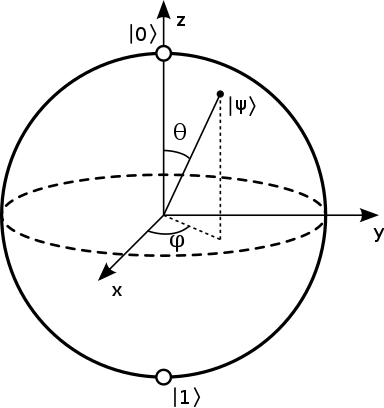
\includegraphics[scale = 0.5]{img/03-esfera_bloch.png}
    \caption{esfera de Bloch para un qubit.}
    Fuente: adaptada de \cite{bloch}
    \label{fig:bloch_sphere}
\end{figure}

Cada punto de la superficie de la esfera representa cada uno de los estados cuánticos puros, en los que se puede encontrar un qubit. Entendiendo como estado cuántico puro el estado que representa completamente la información sobre el sistema en cuestión, es decir, proporciona una descripción completa y detallada de las propiedades cuánticas del sistema. Bajo el marco de la esfera de Bloch, los coeficientes de la ecuación \ref{eq:estado_psi} pueden escribirse en función de los ángulos internos que fijan el estado $\ket{\psi}$, reescribiendo la ecuación por la expresión dada por la ecuación \ref{eq:estado_bloch}.


\begin{equation}
    \ket{\psi} = \cos{\frac{\theta}{2}}\ket{0} + e^{i\phi}\sin{\frac{\theta}{2}}\ket{1}
    \label{eq:estado_bloch}
\end{equation}

La utilidad de la esfera de Bloch queda limitada a solo un qubit, ya que si se quiere describir el estado conjunto $\ket{\psi'}$ que representa el estado global de dos qubits o más, la esfera de Bloch no es útil, dado que el espacio de Hilbert del estado $\ket{\psi'}$ es de dimensión mayor de 2. 

\newpage

El espacio de Hilbert conjunto del $\ket{\psi'}$ que describe el estado de $n$ qubits no es mas el producto tensorial de los espacios individuales de cada qubit. Sea $\mathcal{H}$ el espacio de Hilbert de un qubit, el espacio de Hilbert de $n$ viene dado por $\ket{\psi'} \in \mathcal{H}^{\otimes n}$. Esto hace inviable una representación fidedigna del estado mediante la esfera de Bloch.\\

Realizar operaciones en el paradigma de computación cuántica, consiste en realizar transformaciones a los qubits de tal forma que el vector $\ket{\psi}$ de cada qubit cambie de posición dentro de su esfera de Bloch individual. Sin embargo hay una serie de sutilezas matemáticas que deben exponerse antes de continuar. \\

Dado que trabajamos en el marco de la mecánica cuántica es necesario presentar algunos de los postulados y restricciones matemáticas que se imponen dentro de la propia teoría cuántica \citep{cohen}. En primer lugar, los vectores $\ket{\psi}$ que describen los estados cuánticos de un qubit o conjuntos de qubits, deben ser unitarios. Matemáticamente esta condición viene expresada por la ecuación \ref{eq:unitariedad}. 

\begin{equation}
    |\braket{{\psi}|{\psi}}| = 1
    \label{eq:unitariedad}
\end{equation}

La interpretación física de esta condición implica que los estados cuánticos usados para describir un sistema, es decir, un conjunto de qubits, son completos, contienen toda la información necesaria para describir en su totalidad al sistema. Esta es la razón por la cual, los estados cuánticos puros de un qubit, son aquellos que se encuentran en la superficie de la esfera de Bloch (Figura \ref{fig:bloch_sphere}) ya que son aquellos estados que tienen norma unidad. \\

En segundo lugar, las operaciones que se implementan para operar sobre un estado $\ket{\psi}$ dado deben ser operaciones unitarias. Las operaciones en computación cuántica vienen descritas por operadores, los cuales son objetos matemáticos que realizan transformaciones sobre un estado cuántico dado. Los operadores, deben ser unitarios, esto implica que las transformaciones y operaciones que se realicen sobre un estado $\ket{\psi}$ no deben cambiar la norma del mismo. Matemáticamente la condición de  unitariedad dado un operador $U$ viene dada por la ecuación \ref{eq:operador_unitario}.

\begin{equation}
    U U^{\dagger} = U^{\dagger} U = I
    \label{eq:operador_unitario}
\end{equation}

\newpage

La condición de unitariedad es un restricción que debe cumplir cualquier operación que actúe sobre qubits, con la salvedad de la operación de medida, usada para extraer la información del sistema. En computación cuántica los operadores representan rotaciones dentro de la esfera de Bloch. Los operadores pueden actuar sobre uno o varios qubits de forma simultanea. Dado que estamos operando sobre unidades de información, utilizaremos la palabra puerta cuántica y operador cuántico de forma indistinta durante el presente documento.  \\

Para aliviar el uso de la notación, durante años se ha ido desarrollando notación abstracta la cual permite identificar distintas operaciones que pueden realizarse sobre los qubits \citep{diVincenzo}. Un ejemplo de puerta cuántica es la dada por la expresión \ref{eq:operador_x}.


\begin{equation}
    X = \begin{bmatrix}
    0 & 1 \\
    1 & 0 \\
    \end{bmatrix}
    \label{eq:operador_x}
\end{equation}

La acción de esta puerta, que solo actúa sobre un qubit, cambia o invierte el estado original del qubit. La ecuación \ref{eq:operador_x_estado} da cuenta de la acción de la puerta sobre un qubit en un estado general $\ket{\psi}$.

\begin{equation}
    X \ket{\psi} = X(\alpha\ket{0} + \beta\ket{1}) = \beta\ket{0} + \alpha\ket{1}
    \label{eq:operador_x_estado}
\end{equation}

En términos de la esfera de Bloch, se ha desplazado el estado del qubit desde un punto dado de la superficie de la esfera hasta aquel situado en el punto diametralmente opuesto. El operador que permite realizar un desplazamiento genérico para desplazar el estado $\ket{\psi}$ a cualquier punto de la esfera de Bloch es el dado por la expresión \ref{eq:matriz_bloch}.

\begin{equation}
    \hat{R}(\theta, \phi) = 
    \begin{pmatrix}
        \cos{\frac{\theta}{2}} & -\sin{\frac{\theta}{2}}e^{-i\phi} \\
        \sin{\frac{\theta}{2}}e^{i\phi} & \cos{\frac{\theta}{2}}
    \end{pmatrix}
    \label{eq:matriz_bloch}
\end{equation}

Las expresiones \ref{eq:operador_x} y \ref{eq:matriz_bloch} son puertas cuánticas que tan solo pueden actuar sobre un qubit. Si se quiere implementar tareas de computo en un ordenador cuántico para que pueda llegar a ser una maquina universal cuántica, esto es, poder implementar cualquier tipo de algoritmo cuántico, es necesario introducir puertas cuánticas capaces de actuar sobre 2 qubits. Una de las puertas cuánticas de dos qubits mas conocida es la puerta CNOT, dada por la expresión \ref{eq:cnot}.

\newpage

\begin{equation}
    \text{CNOT} = \begin{bmatrix}
    1 & 0 & 0 & 0 \\
    0 & 1 & 0 & 0 \\
    0 & 0 & 0 & 1 \\
    0 & 0 & 1 & 0 \\
    \end{bmatrix}
    \label{eq:cnot}
\end{equation}

Esta puerta cuántica implementa la operación clásica OR exclusiva. Cualquier operación cuántica que opere sobre $n$ qubits puede descomponerse en operaciones cuánticas de 1 y 2 qubits. Además, existe un conjunto de puertas base que permiten la construcción genérica de cualquier operador unitario, sin embargo, esta familia de puertas base no es univoca. La elección de que conjunto de puertas base se utiliza para realizar la descomposición depende principalmente de la tecnología del hardware cuántico empleado \citep{lin}. \\

Además de las puertas cuánticas, otro operador que es necesario introducir es el operador de energía del sistema cuántico denominado Hamiltoniano \citep{cohen}. El Hamiltoniano es el operador que determina cual es la energía de cada estado posible dentro del espacio de estados del sistema cuántico. El Hamiltoniano rige la evolución temporal del sistema cuántico, dada por la ecuación de Schrödinger representada en la ecuación \ref{eq:schrödinger}.

\begin{equation}
    i\hbar \frac{\partial}{\partial t} |\psi(t)\rangle = \hat{H} |\psi(t)\rangle
    \label{eq:schrödinger}
\end{equation}

El Hamiltoniano no solo rige la evolución temporal del sistema, si no que además establece cuales son los niveles y estados energéticos en los que puede encontrarse un sistema cuántico.

\section{Formulación de problemas de optimización en computación cuántica}

En el paradigma de computación cuántica, la formulación de problemas de optimización no es una tarea trivial, dado que esta debe adaptarse al propio paradigma y a las características únicas de los sistemas cuánticos. En este contexto, es crucial definir cómo representar un problema clásico de optimización, como el problema TSP o el problema Max Cut utilizando conceptos cuánticos como qubits, operadores unitarios y Hamiltonianos.

\newpage

Una vía para modelar problemas de optimización, ya sea de naturaleza cuántica o clásica para poder ser resueltos dentro del paradigma de computación cuántica, es utilizar una formulación binaria del problema \citep{lucas}. Esto permitiría una correspondencia directa entre las variables del problema y los qubits del sistema cuántico. Dado que cada qubit podría representar una variable del problema, y donde el estado del qubit, $\ket{0}$ o $\ket{1}$, representaría el valor de la variable binaria, 0 o 1 respectivamente. \\

Un caso particular de formulación binaria dado un problema, es la denominada formulación Quadratic unconstrained binary optimization, \mbox{QUBO} por sus siglas en inglés. De manera formal si se denota $\Vec{x} = (x_{1}, ..., x_{n})$ como el conjunto de las variables binarias del problema y $f(\Vec{x})$ la función objetivo del problema, un problema tipo \mbox{QUBO} viene representado por la ecuación \ref{eq:qubo}.

\begin{equation}
    f(\Vec{x}) = \sum_{i=1}^{n} \alpha_{i} x_{i} + \sum_{i,j}^{n} \beta_{ij} x_{i} x_{j}
    \label{eq:qubo}
\end{equation}


El problema de optimización se ha transformado en un problema de optimización combinatoria, en el cual se quiere encontrar el vector $\Vec{x}$ que minimice la función $f(\Vec{x})$. Existen una serie de consideraciones a tener en cuenta cuando se modeliza un problema de optimización en una formulación \mbox{QUBO}. En primer lugar, dado que las variables son binarias, es decir, solo pueden tomar el valor $0$ o el valor $1$, implica que $x_{i}^{2} = x_{i}$ para cualquier variable binaria. Otro punto a considerar de la formulación \mbox{QUBO} es que no permite la existencia de restricciones. Sin embargo, en muchos de los problemas, la existencia de restricciones es algo común. Una forma habitual de incorporar las restricciones a la función objetivo $f(\Vec{x})$ de tal manera que formalmente las restricciones se eliminen aunque si estén incorporadas, es incluir las restricciones como términos de penalización adicionales dentro de la función $f(\Vec{x})$ \citep{glover}. De esta manera, si una solución no satisface una restricción, se eleva artificialmente el valor de la función objetivo. Una restricción típica puede ser la dada por la expresión \ref{eq:linear_restriction}.

\begin{equation}
    \sum_{i=1}^{n}c_ix_i = C, \; \; c_i \in \mathbb{Z} 
    \label{eq:linear_restriction}
\end{equation}


Esta restricción se incorpora a la función $f(\Vec{x})$ como un termino adicional resultando en una nueva función objetivo dada por la ecuación \ref{eq:qubo_restriction}.

\newpage

\begin{equation}
    f(\Vec{x}) = \sum_{i=1}^{n} \alpha_{i} x_{i} + \sum_{i,j}^{n} \beta_{ij} x_{i} x_{j} + \lambda_0(\sum_{i=1}^n c_ix_i-C)^2
    \label{eq:qubo_restriction}
\end{equation}

El parámetro $\lambda_0$ es un hiperparametro, denominado constante de Lagrange, cuyo valor se determina de forma heurística, de tal forma que si una solución no satisface la restricción se eleve ``moderadamente'' la energía de la función objetivo. Otras restricciones mas complicadas como aquellas que poseen desigualdades, son mas complejas de introducir, ya que usualmente se requiere de variables adicionales, denominadas variables slack, para transformar la restricción de desigualdad en una restricción de igualdad, para posteriormente ser introducida como termino de penalización dentro de la función objetivo. Sea una restricción de desigualdad como la dada por la expresión \ref{eq:restriction_inequality}.


\begin{equation}
    \sum_{i=1}^nl_ix_i \leq B, \; \; l_i \in \mathbb{Z}
    \label{eq:restriction_inequality}
\end{equation}

Esta restricción se transforma en una restricción de igualdad dada por la expresión \ref{eq:restriction_nonequal_equal}.

\begin{equation}
    B - \sum_{i=1}^n l_ix_i - S = 0
    \label{eq:restriction_nonequal_equal}
\end{equation}

Donde $S$ toma valores cuyo rango es $0 \leq S \leq B - min_x \sum_{i=1}^n l_ix_i$. Para transformar $S$ en variables binarias, se expresa $S$ como una suma de variables binarias tal y como se observa en la expresión \ref{eq:s_binary}.

\begin{equation}
    S = \sum_{k=0}^{N-1}2^ks_k
    \label{eq:s_binary}
\end{equation}

Introduciendo \ref{eq:s_binary} en  \ref{eq:restriction_nonequal_equal} e introduciendo el resultado en \ref{eq:qubo}, conseguimos incluir la restricción de desigualdad como un termino de penalización tal y como se puede ver en la ecuación  \ref{eq:final_equation}.

\begin{equation}
    f(\Vec{x}) = \sum_{i=1}^{n} \alpha_{i} x_{i} + \sum_{i,j}^{n} \beta_{ij} x_{i} x_{j} + \lambda_1 (B - \sum_{i=1}^n l_ix_i - \sum_{k=0}^{N-1}2^ks_k)^2,
    \label{eq:final_equation}
\end{equation}

Se han desarrollado metodologías alternativas \citep{montañez23} donde las restricciones de desigualdad se introducen como términos de penalización en la función objetivo $f(\Vec{x})$ sin requerir variables adicionales para tal objetivo. \\

En resumen, la modelización de problemas de optimización mediante formulación \mbox{QUBO} es una forma habitual de proceder cuando se pretende formular un problema de optimización de tal forma pueda ser computado dentro del paradigma de computación cuántico. Existen formulaciones en donde se permite la existencia dentro de la función objetivo $f(\Vec{x})$, de términos de orden superior a los cuadráticos. La formulación del problema de optimización es un paso clave dentro de flujo de trabajo.

\subsection{Problema objetivo}
\label{sub:problem_target}

Un problema ya mencionado anteriormente, el cual es uno de los mas utilizados dentro de la comunidad de computación cuántica para presentar resultados de nuevos algoritmos cuánticos, es el problema NP-Duro denominado como Max Cut \citep{heal}. Este será el problema usado para presentar los resultados obtenidos en el presente trabajo. \\

Dado un grafo no dirigido $ G = (V, E) $ con un conjunto de vértices $ V $ y un conjunto de aristas $ E $, el objetivo del problema Max Cut es encontrar una partición de los vértices $ V $ en dos subconjuntos disjuntos $ A $ y $ B $ tal que el número de aristas que cruzan entre $ A $ y $ B $, es decir, las aristas que tienen un extremo en $ A $ y el otro extremo en $ B $, sea máximo. Estas aristas se conocen como el corte del grafo, y el tamaño del corte es el número de aristas que cruzan entre $ A $ y $ B $. De forma visual, el problema Max Cut viene representado por la Figura \ref{fig:max_cut_problem}. 


\begin{figure}[!h]
    \centering
    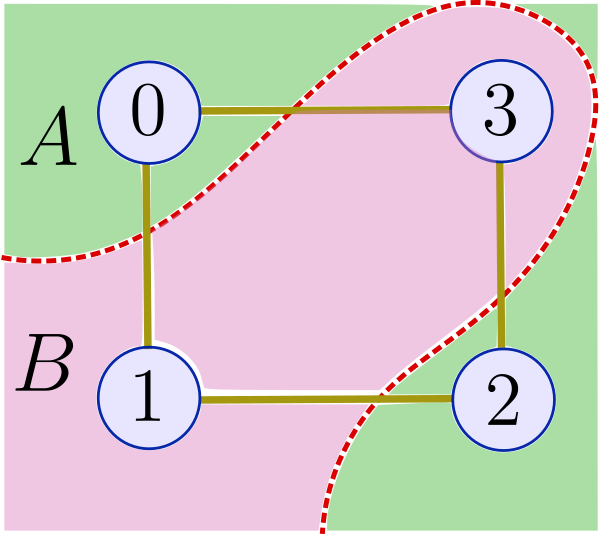
\includegraphics[scale = 0.8]{img/03-max_cut_problem.png}
    \caption{representación del problema Max Cut}
    Fuente: adaptada de \cite{pn}.
    \label{fig:max_cut_problem}
\end{figure}

\newpage

El problema Max Cut, admite una formulación \mbox{QUBO} natural dada por la expresión \ref{eq:max_cut_problem_max}.

\begin{equation}
    \text{Maximizar} \quad f(\Vec{x}) = \sum_{(i,j) \in E} (x_i + x_j -2x_ix_j)
    \label{eq:max_cut_problem_max}
\end{equation}

La expresión \ref{eq:max_cut_problem_max} modeliza el problema que se desea resolver, donde el valor de las variables binarias marca a que subconjunto pertenece cada uno de los vértices $V$ del grafo, siendo los de valor $0$ el primer subconjunto y los de valor $1$, los del segundo subconjunto. \\


Dado que se desea maximizar la expresión \ref{eq:max_cut_problem_max}, se necesita que para  el máximo número de aristas posible, el término $x_i + x_j -2 x_i x_j$  sea positivo no nulo y esto solo ocurre cuando las variables $x_i$ y $x_j$ toman valores diferentes. Para ello, necesariamente $x_i$ y $x_j$ deben pertenecer a subconjuntos distintos, ya que es la única combinación posible en la cual el termino del sumando es no nulo y positivo. \\

Tal y como está definido \ref{eq:max_cut_problem_max}, se trata de un problema de maximización, sin embargo si deseamos tratar el problema como un problema de minimización, podemos añadir un signo negativo global a la función, aprovechando la equivalencia de $max\{ f(x)\} = - \; min\{ - f(x) \}$. Esto transforma el problema Max Cut en un problema de minimización, tal y como viene dado en la expresión \ref{eq:max_cut_problem_min}, lo cual es mas adecuado para nuestros propósitos.

\begin{equation}
    \text{Minimizar} \quad f(\Vec{x}) = - \sum_{(i,j) \in E} (x_i + x_j - 2x_i x_j)
    \label{eq:max_cut_problem_min}
\end{equation}

La expresión objetivo se convierte ahora en una función cuyo mínimo, en valor absoluto, representa el valor solución del problema. El problema Max Cut, aunque simple, es un problema base que posee aplicaciones directas en ámbitos como la inteligencia artificial o el diseño de circuitos. El problema Max Cut tiene una representación dual, ya sea en forma de grafo o en forma de las expresiones \ref{eq:max_cut_problem_max} y \ref{eq:max_cut_problem_min}. Con el objetivo de generar un conjunto suficientemente grande de problemas Max Cut, se va a utilizar un generador de grafos de tipo Erdös–Rényi \citep{li}. Un grafo de tipo Erdös $G(n,p)$, es aquel grafo que posee $n$ vértices con una probabilidad de conexión con el resto de vértices de $p$. Este tipo de grafos permite, dado un tamaño y una probabilidad de conexión, generar un conjunto grande de problemas Max Cut. 

\newpage


\section{Algoritmos variacionales cuánticos}

En está sección se presentan la clase de algoritmos cuánticos utilizados en el desarrollo de trabajo. Los algoritmos cuánticos variacionales \citep{cerezo} conforma un subconjunto de algoritmos cuánticos orientados a la resolución de problemas de optimización. Uno de los conceptos centrales en este tipo de algoritmos cuánticos es el de Hamiltoniano, ya que estos algoritmos están orientados a encontrar cual es el estado de mínima energía del sistema, es decir, cual es el vector o vectores propios del Hamiltoniano de menor energía. \\


El Hamiltoniano no es un operador unitario, a diferencia de las puertas cuánticas, dado que el objetivo de este operador no es actuar sobre los qubits para cambiar su estado, si no conocer la energía del estado en el que se encuentra el sistema cuántico. Formalmente, la acción del Hamiltoniano, $H$ sobre un estado del sistema $\ket{\psi}$ viene dado por la ecuación \ref{eq:autovalor_h}.

\begin{equation}
    H \ket{\psi} = E \ket{\psi}
    \label{eq:autovalor_h}
\end{equation}

La ecuación \ref{eq:autovalor_h} se denomina ecuación de autovalores y permite obtener la energía de cada estado $\ket{\psi}$ del sistema. Este hecho permite mostrar una analogía entre la ecuación de autovalores con la evaluación de una función \mbox{QUBO} $f(\Vec{x})$, para un conjunto de valores dados de las variables binarias. Dado un vector $\ket{\psi}$ la ecuación \ref{eq:autovalor_h} nos devuelve el valor $E$ asociado para un $H$ especifico, del mismo modo que dado un vector de variables fijadas $\Vec{x}_{0}$, la evaluación $f(\Vec{x}_0)$ nos devuelve el valor de $f(\Vec{x})$ en el estado $\Vec{x}_0$. Se puede establecer una relación matematica entre las formulaciones \mbox{QUBO} clásicas de los problemas y formulaciones cuánticas mediante Hamiltonianos. Existe un mapeo directo de la formulación \mbox{QUBO} a una formulación cuántica mediante Hamiltonianos denominada formulación Ising. La transformación entre formulaciones \mbox{QUBO}-Ising viene dada por la expresión \ref{eq:qubo_ising}.

\begin{equation}
    x_{i} \longrightarrow \frac{1 - Z_{i}}{2}
    \label{eq:qubo_ising}
\end{equation}

Donde $Z_{i}$ representa el operador o puerta cuántica de Pauli $Z$ actuando sobre el qubit i-ésimo. Se pasa de un problema de variables binarias con valores $0$ y $1$ en formulación \mbox{QUBO}, a variables con valores $1$ y $-1$, en formulación Ising. Esta regla permite traducir de forma directa un problema \mbox{QUBO}, escrito en terminos de variables binarias clásicas, a un Ising, escrito en terminos de operadores cuánticos \citep{lucas}.

\newpage

En formulación Ising el problema Max Cut presentado en el apartado \ref{sub:problem_target} viene dada por la expresión \ref{eq:problem_ising_target}, en la versión de minimización.

\begin{equation}
    \text{Minimizar} \quad H =  - \frac{1}{2}\sum_{(i,j) \in E} (1 - Z_i Z_j)
    \label{eq:problem_ising_target}
\end{equation}

Podemos ahora introducir el funcionamiento de los algoritmos cuánticos variacionales una vez entendida la relación entre la formulación de Hamiltonianos y la formulación  \mbox{QUBO} de problemas clásicos. Los algoritmos variacionales cuánticos hacen uso del denominado principio variacional de Rayleigh-Ritz \citep{fernandez}. El principio viene expresado matemáticamente por la ecuación \ref{eq:variational_principle}.

\begin{equation}
    \bra{\psi} H \ket{\psi} \geq E_{0}
    \label{eq:variational_principle}
\end{equation}

El principio variacional determina que el valor esperado del Hamiltoniano, la energía del sistema que es observada, se minimiza cuando $\ket{\psi}$ representa el estado fundamental del sistema cuántico. Para cualquier otro estado genérico $\ket{\psi_{i}}$ el valor esperado, $E_{i}$, siempre es mayor que el valor mínimo $E_{0}$. Esto permite establecer un criterio de búsqueda para encontrar el estado $\ket{\psi}$ que representa el estado fundamental del sistema, ya que será este estado el que minimice la ecuación \ref{eq:variational_principle}. Los algoritmos variacionales cuánticos hacen uso de este principio para encontrar el estado $\ket{\psi}$ que minimiza el valor esperado del Hamiltoniano. En terminos clásicos esto es equivalente a encontrar el vector de parámetros $\Vec{x}$ que minimiza la función de coste $f(\Vec{x})$. \\

El primer algoritmo variacional cuántico propuesto, fue el denominado  Variational Quantum Eigensolver, o VQE \citep{peruzzo} por sus siglas en inglés. El flujo de trabajo del algoritmo VQE puede resumirse mediante la Figura \ref{fig:vqe}. El algoritmo VQE como algoritmo híbrido clásico-cuántico consta de dos partes bien diferenciadas. En un primer paso, el ordenador cuántico prepara un estado cuántico $\ket{\psi(\Vec{\theta})}$ que depende de un conjunto de parámetros $\Vec{\theta}$. Esto se consigue mediante los denominados \mbox{PQC} o circuitos cuánticos parametrizados, los cuales son una secuencia de puertas cuánticas que actúan sobre los qubits y que dependen de un conjunto de parámetros $\Vec{\theta}$.

\newpage

\begin{figure}[!ht]
    \centering
    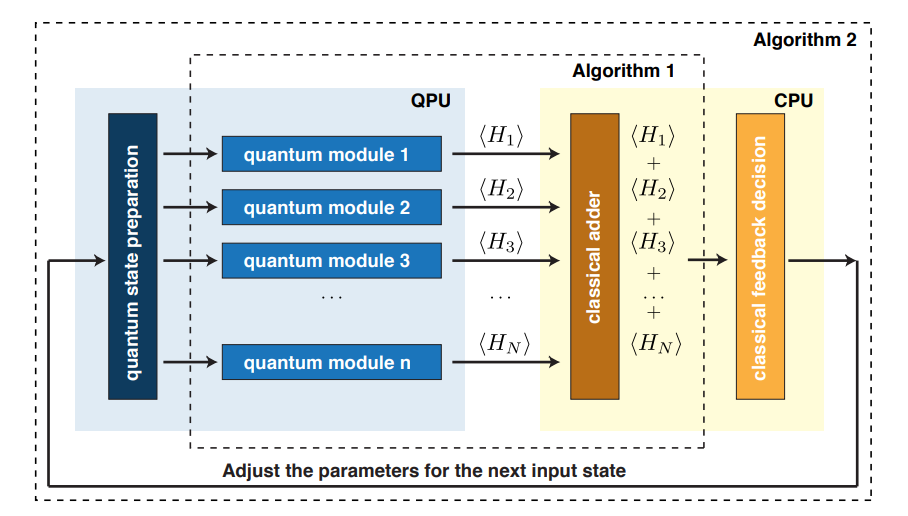
\includegraphics[scale = 0.7]{img/03-vqe_workflow.png}
    \caption{flujo de trabajo del algoritmo VQE.}
    Fuente: adaptada de \cite{peruzzo}.
    \label{fig:vqe}
\end{figure}

La construcción del estado $\ket{\psi(\Vec{\theta})}$ viene dado por la expresión \ref{eq:pqc}.

\begin{equation}
    |\psi(\boldsymbol{\Vec{\theta}}) \rangle = U(\boldsymbol{\Vec{\theta}}) |0\rangle^{\otimes n}
    \label{eq:pqc}
\end{equation}

Donde $U(\boldsymbol{\Vec{\theta}})$ es el operador unitario que representa la acción del circuito cuántico parametrizado sobre los \textit{n} qubits, que se encuentran todos ellos en el estado $\ket{0}$. La acción del \mbox{PQC} se realiza descomponiendo el operador global en términos de operadores o puertas cuánticas de 1 y 2 qubits, tal y como se ve en la expresión \ref{eq:pqc_descompuesto}.

\begin{equation}
    U(\boldsymbol{\Vec{\theta}}) = U_n(\theta_n) U_{n-1}(\theta_{n-1}) \cdots U_1(\theta_1)
    \label{eq:pqc_descompuesto}
\end{equation}

Una vez el ordenador cuántico ha preparado el sistema en el estado $\ket{\psi(\Vec{\theta})}$, el siguiente paso es el calculo del valor esperado del Hamiltoniano que codifica el problema que nos interesa resolver. Una vez calculado el valor esperado del Hamiltoniano, un ordenador clásico analiza el resultado y calcula un nuevo vector de parámetros $\Vec{\theta'}$ para construir un nuevo estado $\ket{\psi(\Vec{\theta'})}$. Este nuevo estado $\ket{\psi(\Vec{\theta'})}$ a su vez se utiliza para calcular el valor del Hamiltoniano para posteriormente actualizar los parámetros $\Vec{\theta}$ del circuito cuántico parametrizado.

\newpage

Realizando este proceso de forma iterativa, se llegará en un numero finito de pasos a un circuito cuántico parametrizado que genere un estado $\ket{\psi(\Vec{\theta_{final}})}$, el cual minimiza el valor esperado del Hamiltoniano. Por el principio variacional, este vector representa el estado que minimiza la energía del sistema, o lo que es lo mismo, el estado fundamental. Se ha encontrado así el estado que minimiza el Hamiltoniano o en terminos de formulación \mbox{QUBO}, se ha encontrado el valor de las variables binarias que minimiza la función de coste $f$. \\

Posterior a la aparición del algoritmo VQE, numerosos algoritmos cuánticos variacionales han surgido en la literatura académica. Uno de los mas destacados es el algoritmo Quantum Approximate Optimization Algorithm, o QAOA \citep{farhi} por sus siglas en inglés. La diferencia principal entre el algoritmo QAOA y el algoritmo VQE es el tipo de circuito cuántico parametrizado se usa para la preparación del estado  $\ket{\psi(\Vec{\theta})}$. En el algoritmo QAOA el circuito encargado de construir un estado parametrizado $\ket{\psi(\Vec{\theta})}$ viene dado por la expresión \ref{eq:pqc_qaoa}.


\begin{equation}
    U(\vec \gamma,\vec \beta)=\prod_{k=1}^p e^{-i \gamma_k H_C} e^{- i \beta_k H_M}
    \label{eq:pqc_qaoa}
\end{equation}

Donde $H_C$ hace referencia al Hamiltoniano problema y $H_M=-\sum_{i=1}^n X_i$, al denominado Hamiltoniano de mezcla. El productorio implica la aplicación de $p$ capas, de los operadores $e^{-i \gamma_k H_C}$ y $e^{- i \beta_k H_M}$, que actúan sobre el estado base. En la Figura \ref{fig:qaoa_layers} se puede observar la estructura de $p$ capas para construir un estado parametrizado.

\begin{figure}[!ht]
    \centering
    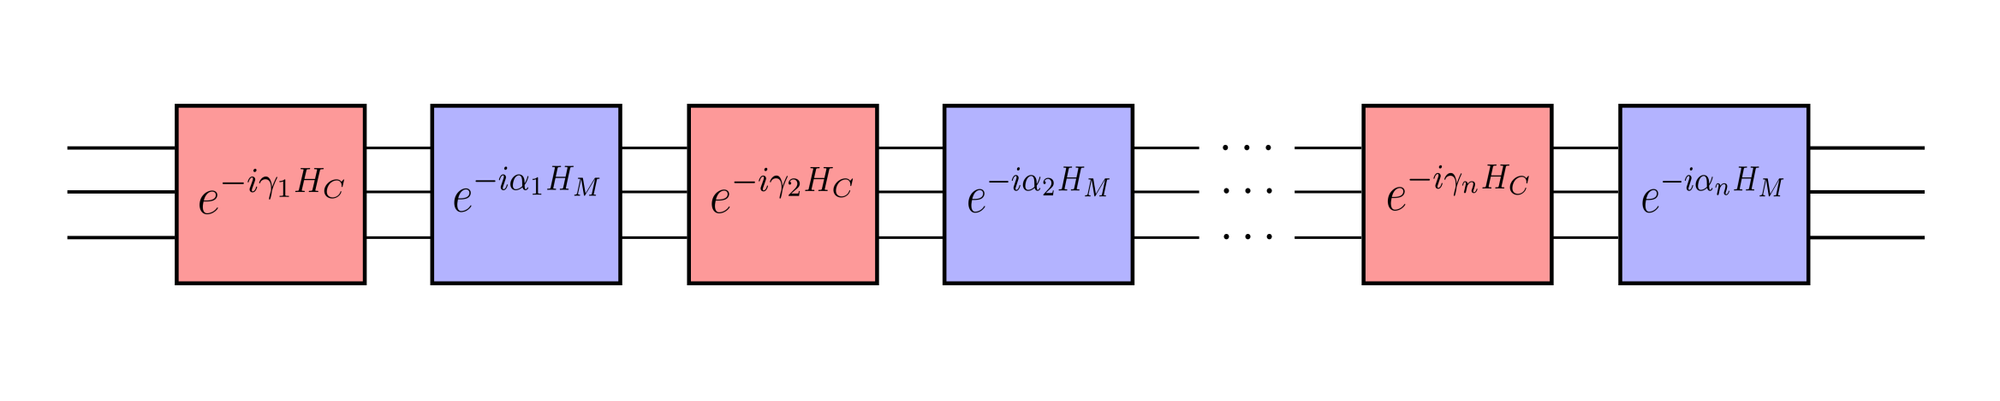
\includegraphics[scale = 0.4]{img/03-qaoa_layers.png}
    \caption{esquema de \mbox{PQC} para el algoritmo QAOA.}
    Fuente: adaptada de \cite{jack}
    \label{fig:qaoa_layers}
\end{figure}

Los operadores expresados como exponenciales complejas pueden implementarse a través de una secuencia de puertas cuánticas de 1 y 2 qubits. El resto del funcionamiento de algoritmo es equivalente al del algoritmo VQE. 

\newpage

Una vez construido el estado parametrizado, $\ket{\psi(\Vec{\gamma}, \Vec{\beta})}$, se evalúa el valor esperado del Hamiltoniano para posteriormente, gracias a un ordenador clásico que implementa un optimizador, se actualizan el conjunto de parámetros para reducir el valor esperado de la energía del sistema. En general cualquier algoritmo cuántico variacional consta de tres componentes principalmente. 

\begin{itemize}
    
    \item Circuito cuántico parametrizado o \mbox{PQC}: conjunto y estructura de puertas cuánticas utilizadas para preparar el estado inicial en un ordenador cuántico. Contiene los parámetros variacionales que pueden ajustarse durante el proceso de optimización.

    \item Optimizador clásico: el optimizador clásico se encarga de ajustar los parámetros variacionales en el \mbox{PQC} para minimizar la función de coste. Utiliza técnicas clásicas de optimización para encontrar el conjunto óptimo de parámetros que produzcan el resultado deseado.

    \item Función de coste: la función de coste cuantifica el objetivo que el algoritmo variacional pretende optimizar. Evalúa la calidad de la salida obtenida del circuito cuántico. El objetivo es minimizar la función de coste ajustando los parámetros variacionales.
    
\end{itemize}

Puede afirmarse que tanto el algoritmo VQE como el algoritmo QAOA son los algoritmos fundacionales dentro de los algoritmos cuánticos variacionales. Numerosos algoritmos han surgido como versiones modificadas y mejoradas tanto del algoritmo VQE como del algoritmo QAOA. Por ejemplo, el algoritmo F-VQE \citep{amaro} implementa un optimizador clásico nativo basado en el descenso del gradiente. Otras versiones modificadas del algoritmo VQE como el algoritmo MOVCO \citep{luis}, implementan dos funciones de coste que deben ser optimizadas de forma simultánea. Así mismo, también se han desarrollado numerosas versiones del algoritmo QAOA, como el ADAPT-QAOA \citep{zhu}, en el cual cada una de las capas del QAOA se optimiza de forma iterativa y dónde el circuito cuántico parametrizado se construye de forma dinámica. \\

El objetivo de todas las versiones surgidas posteriores a los algoritmos VQE y QAOA originales tratan de mitigar y superar las deficiencias que existen en esta clase de algoritmos. Los problemas que presentan esta clase de algoritmos están asociados principalmente a que no aseguran la convergencia a soluciones que sean óptimos globales.

\newpage

Otro problema asociado se debe al efecto de \textit{Barren Plateaus} \citep{mcClean}, un fenómeno por el cual las superficies de energía, de las funciones de costo, exhiben zonas casi planas en el paisaje de la función objetivo. Esto significa que los gradientes de la función (es decir, las direcciones en las que cambia más rápidamente la función) se vuelven extremadamente pequeños o cercanos a cero en muchas partes del espacio de parámetros. La presencia de estas \textit{Barren Plateaus} puede ser problemática para los algoritmos de optimización cuántica, ya que los métodos estándar que confían en la exploración guiada por gradientes pueden volverse ineficaces. 

\section{Introducción a tensor networks}


Tensor networks \citep{orus} es una técnica y herramienta fundamental en física teórica y materia condensada que permite representar estados cuánticos complejos y realizar cálculos eficientes en sistemas de muchas partículas. En una tensor network, un estado cuántico se descompone en un conjunto de tensores interconectados, donde cada tensor representa una parte localizada del sistema. La estructura y disposición de estos tensores captura las correlaciones cuánticas entre las distintas partes del sistema. \\

La utilidad de las tensor networks radica en su capacidad para manejar estados cuánticos de alta dimensionalidad de manera eficiente. Por ejemplo, en sistemas cuánticos con muchas partículas, representar directamente el estado completo sería computacionalmente prohibitivo debido a la explosión combinatoria de las dimensiones. Sin embargo, mediante una representación basada en tensor networks, podemos enfocarnos en las correlaciones locales significativas y omitir aquellas que son menos relevantes, reduciendo así el coste computacional. Es decir, permite un manejo eficiente de sistemas cuánticos grades que bajo otro formalismo no sería factible. \\


Las tensor networks se han aplicado con éxito en diversas áreas, incluida la simulación de materia condensada y sistemas cuánticos, donde permiten estudiar propiedades como la energía, la magnetización y las funciones de correlación. Además, han encontrado aplicaciones en el campo emergente del aprendizaje automático \citep{chen}. 

\newpage

Dado un estado cuántico $\ket{\psi}$, se puede expresar dicho estado cuántico en términos de una combinación lineal de los estados base, que para el caso particular de un solo qubit, son los estados $\ket{0}$ y $\ket{1}$. La expansión genérica de un estado de $N$ qubits viene dado por la expresión \ref{eq:psi_expansion}.

\begin{equation}
    \ket{\psi} = \sum_{i_1, i_2, ...,i_N} C_{i_1, i_2, ...,i_N} \ket{i_1}\otimes\ket{i_2}\otimes...\otimes \ket{i_N}
    \label{eq:psi_expansion}
\end{equation}

Donde los estados $\ket{i_1}\otimes\ket{i_2}\otimes...\otimes \ket{i_N}$ son los estados de la base del estado $\ket{\psi}$ expresado en términos de los estados base $\ket{i_s}$ de cada uno de los qubits del sistema. Los coeficientes $C_{i_1, i_2, ...,i_N}$ de la expansión puede entenderse como un tensor que posee $N$ índices, cada uno de los cuales puede tomar valores distintos. Gráficamente puede representarse en el formalismo de tensor networks al tensor $C$ tal y como se observa en la Figura \ref{fig:orus}.

\begin{figure}[!ht]
    \centering
    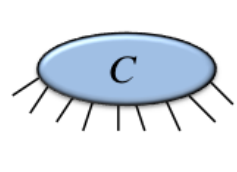
\includegraphics[scale = 0.8]{img/03_tensor_coeficientes.png}
    \caption{representación del tensor de coeficientes $C$  de la expansión del estado $\ket{\psi}$.}
    Fuente: adaptada de \cite{orus}
    \label{fig:orus}
\end{figure}

En la Figura \ref{fig:orus} cada una de las patas del tensor $C$ representa cada uno de los índices del tensor. Sin embargo, la dimesionalidad del tensor $C$ es enorme para sistemas cuánticos de muchos qubits o partículas, por lo que es necesario descomponer el tensor $C$ en terminos de tensores mas pequeños para poder trabajar de forma eficiente con el. Formalmente y siguiendo la regla de índices de Einstein \citep{ahlander}, un tensor $C$ puede expresarse como producto de varios tensores de menor rango, menor dimesionalidad, tal y como se muestra en la expresión \ref{eq:contracction}.

\begin{equation}
    C_{i j} = \sum_{\alpha} A_{i  \alpha} B_{j \alpha} = A_{i  \alpha} B^{j \alpha}
    \label{eq:contracction}
\end{equation}

Esto permite expresar un tensor arbitrariamente grande en terminos de una descomposición de tensores de menor dimensión. Graficamente, esta descomposición puede dar lugar a distintas redes de tensores, dado que la descomposición de un tensor no es única. En la Figura \ref{fig:c_descomposition} pueden observarse distintas posibles descomposiciones del tensor $C$ en terminos de tensores de menor dimesionalidad.


\begin{figure}[!ht]
    \centering
    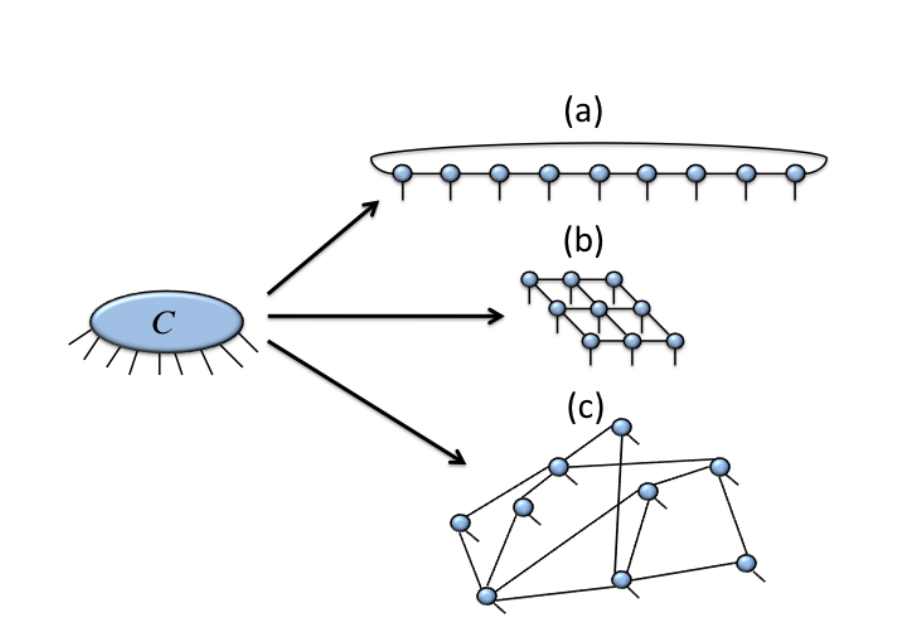
\includegraphics[scale = 0.7]{img/03-tensor_descomposicion.png}
    \caption{descomposición del tensor $C$ en distintas redes tensoriales.}
    Fuente: adaptada de \cite{orus} 
    \label{fig:c_descomposition}
\end{figure}

\newpage

Las patas internas, aristas que unen entre sí a los tensores, de la red tensorial representan los índices de los tensores que se contraen, tal y como dicta la ecuación \ref{eq:contracction} para poder obtener el tensor $C$. Por otro lado, las patas abiertas, representan los índices físicos del tensor $C$, las patas originales del tensor que no aparecen por la descomposición, ya que al contraer la red, estos índices sobreviven. La figura $(a)$ de la imagen \ref{fig:c_descomposition} representa un tipo especifico de descomposición denominada Matrix Product State, o MPS por sus siglas en inglés, y es una representación especialmente conveniente para simular sistemas en computación cuántica. Bajo la representación MPS, cada tensor de la red corresponde con un qubit del sistema cuántico, donde cada índice o pata abierta corresponde con la dimensión física del qubit. En el trabajo desarrollado en este documento se hará uso de la representación MPS para realizar simulaciones eficientes de sistemas cuánticos. Es importante tener en cuenta, que bajo este formalismo podemos realizar simulaciones eficientes de sistemas cuánticos, pero simulaciones no exactas. El parámetro que dicta que tan buena es la aproximación entre la simulación aproximada y la exacta es la dimensión $D$ de los índices internos de la red de tensores. Cuanto mayor sea el valor de $D$ mejor será la aproximación. La dimensión de los índices internos determinan la cantidad de correlaciones que la red de tensores es capaz de capturar del sistema cuántico. Un sistema cuántico con correlaciones entre los qubits baja, requiere un valor bajo de $D$ para poder ser simulado de forma suficientemente buena. En la Figura \ref{fig:mps_hilbert_space} podemos ver como la dimensión interna de los índices de la red impacta en el tamaño del espacio de Hilbert total que es capaz de capturar en la representación MPS.


\begin{figure}[!ht]
\centering
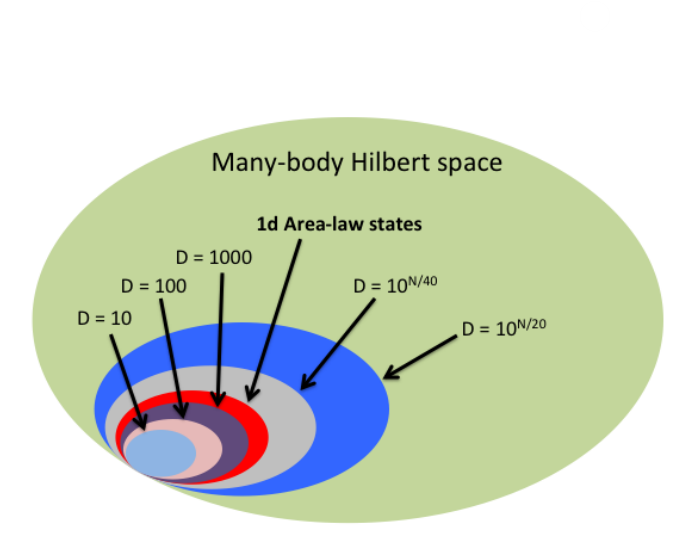
\includegraphics[scale = 0.55]{img/03-mps_espacio_hilbert.png}
\caption{subespacio de Hilbert que es capaz de representar una red MPS en función de la dimensión interna $D$ para un sistema de $N$ qubits.}
Fuente: adaptada de \cite{orus} 
\label{fig:mps_hilbert_space}
\end{figure}

Sin embargo, aumentar la dimensión interna de la red de tensores conlleva un coste computacional, ya que por la ecuación \ref{eq:contracction}, el aumento de la dimensión implica un aumento en el numero de productos y sumas a realizar cuando se quieren contraer dos tensores de la red. Es necesario fijar una dimensión interna suficientemente alta para realizar simulaciones fidedignas pero que no impliquen un coste computacional prohibitivo. De esta forma podemos realizar simulaciones eficientes de estados cuánticos. \\

Bajo el formalismo de tensor networks, las puertas cuánticas de un qubit se entienden como matrices, tensores de dos índices, las cuales pueden operar sobre estados cuánticos en forma de MPS simplemente contrayendo el índice de entrada de la puerta cuántica sobre el índice físico del tensor, qubit, correspondientes del estado MPS. Para el caso de puertas de dos qubits, tenemos tensores de cuatro índices, dos de entrada y dos de salida. \\

\newpage

Además de entender como representar estados cuánticos de forma eficiente bajo el formalismo de tensor networks, es necesario entender también como codificar Hamiltonianos en este paradigma. Existe un objeto en tensor networks el cual es una extensión natural de los estados MPS, denominados Matrix Product Operator o MPO, por sus siglas en inglés. Un operador MPO es una tensor network donde cada tensor tiene dos patas no contraídas, así como dos patas internas que conectan con los tensores vecinos en forma de cadena, tal y como puede visualizarse en la Figura \ref{fig:mpo}.


\begin{figure}[!ht]
    \centering
    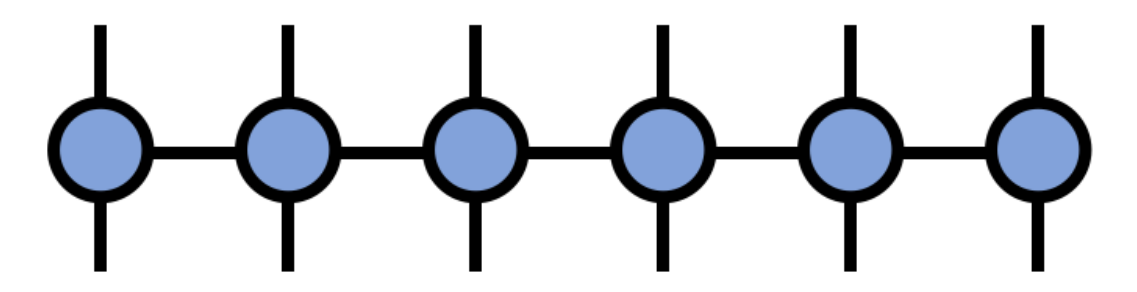
\includegraphics[scale = 0.35]{img/03-mpo.png}
    \caption{representación de un MPO}
    Fuente: adaptada de \cite{tn} 
    \label{fig:mpo}
\end{figure}

De igual manera que un estado MPS representa un estado cuántico, el MPO representa un operador cuántico. Existen diversas formas de construir el MPO a partir de un Hamiltoniano. Para Hamiltonianos con interacciones no locales, es decir Hamiltonianos donde los qubits interactúan entre sí, independientemente de si son vecinos o no, la construcción del operador MPO no es trivial. Se han propuesto reglas \citep{fröwis} para poder construir de forma eficiente MPO's que representen Hamiltonianos genéricos que contengan interacciones no locales. De forma general un operador se puede describir a través de la expresión \ref{eq:operator}.

\begin{equation}
    H = \sum_{i} \sum_{i'} C_{i_1 i_2 \ldots i_L}^{i'_1 i'_2 \ldots i'_L} \left| i_1 i_2 \ldots i_L \right\rangle \left\langle i'_1 i'_2 \ldots i'_L \right|
    \label{eq:operator}
\end{equation}

De forma análoga a lo realizado para los estados $\ket{\psi}$, podemos descomponer el tensor $ C_{i_1 i_2 \ldots i_L}^{i'_1 i'_2 \ldots i'_L}$ en tensores de menor dimensión. Esta descomposición del tensor, que representa en el operador Hamiltoniano, en tensores de menor dimensión es lo que da lugar a la representación en forma de MPO de un operador tal y como hemos visto en la figura \ref{fig:mpo}. \\


Bajo el paradigma de tensor networks, la ecuación \ref{eq:autovalor_h} viene dada por la contracción del estado $\ket{\psi}$ sobre el MPO que representa el operador $H$. En la Figura \ref{fig:mpo_to_mps} se observa en forma tensorial la ecuación de autovalores dada por la acción del MPS sobre el MPO.

\newpage

\begin{figure}[!ht]
    \centering
    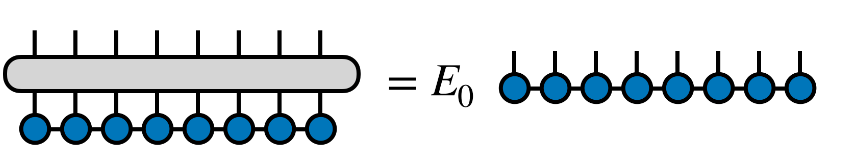
\includegraphics[scale = 0.65]{img/03-mpo_to_mps.png}
    \caption{representación en forma tensorial de la ecuación de autovalores}
    Fuente: adaptada de \cite{tn} 
    \label{fig:mpo_to_mps}
\end{figure}

Los conceptos de MPS y MPO para la representación de estados cuánticos y operadores, respectivamente, son las ideas más importantes, dentro del campo de las tensor networks, para el desarrollo del trabajo realizado. 


\section{Computación cuántica en entornos industriales}

Es necesario contextualizar el estado teórico de los algoritmos cuánticos, de los cuales se pretenden hacer uso, con el estado del hardware en los cuales deben ejecutarse. Actualmente nos encontramos en la época denominada de ordenadores ruidosos de escala intermedia \citep{preskill} o NISQ por sus siglas en inglés. Las computadoras cuánticas en la era NISQ están limitadas en términos de la cantidad de qubits que poseen y la calidad de las operaciones cuánticas que pueden implementar. Esto significa que estas máquinas no están completamente libres de errores y tienen una capacidad de cómputo limitada en comparación con lo que se espera en sistemas cuánticos futuros. Los qubits en las máquinas NISQ son susceptibles a errores debido al ruido y la decoherencia cuántica. Estos errores pueden surgir debido a fluctuaciones ambientales y limitaciones tecnológicas en el control de los sistemas cuánticos. \\

La decoherencia es el fenómeno físico por el cual un estado cuántico $\ket{\psi}$ se destruye después de un tiempo dado, es decir, el tiempo de coherencia es la cantidad de tiempo que un estado cuántico $\ket{\psi}$ permanece, es decir, el tiempo en el que el sistema cuántico conserva la información. Actualmente el tiempo de coherencia de los ordenadores cuánticos impone una restricción fuerte en términos de la profundidad de los circuitos cuánticos que pueden ejecutarse. Dado que la profundidad del circuito no puede superar el tiempo de coherencia, esto provoca que los circuitos deban ser poco profundos y la cantidad de puertas cuánticas que se apliquen sean limitadas. Esto limita a su vez los algoritmos cuánticos que puede ser ejecutados actualmente en ordenadores cuánticos, siendo los algoritmos cuánticos variacionales de los pocos tipos de algoritmos que actualmente pueden ejecutarse de forma relativamente fiable en las plataformas cuánticas \citep{bharti}. \\

Otro problema asociado al estado actual del hardware se debe al costo económico por el acceso y uso de plataformas cuánticas reales. El número de ordenadores cuánticos disponibles es limitado. Esto supone que el acceso al uso y ejecución de estos ordenadores conlleva un gran costo económico asociado, por lo que utilizar algoritmos cuánticos para la resolución de problemas que requieran de un uso intensivo de ordenadores cuánticos puede ser inviable en términos de coste económico. 






\chapter{Objetivos}

\section{Objetivo general}

El objetivo principal de este proyecto es el desarrollo de un esquema de preprocesado basado en tensor networks que permita superar las deficiencias presentes en los protocolos existentes. El nuevo esquema de preprocesado está basado en la creación de estados de Gibbs puros.

\section{Objetivos específicos}

Los objetivos planteados para el trabajo han sido los siguientes:

\begin{itemize}
    
    \item Comprender e implementar algoritmos de tensor networks que puedan ser de interés en el campo de la computación cuántica.
    
    \item Implementar un método híbrido de tensor networks y computación cuántica para la resolución de problemas de optimización.
   
    \item Implementar un método híbrido novedoso, basado en los estados cuánticos de Gibbs, que supere a los presentes en el estado del arte.
     
    \item Realizar comparativas de rendimiento entre el método propuesto y el método presente en el estado del arte.

\end{itemize}

\section{Hipótesis planteadas}

La hipótesis planteada para este trabajo y que recoge los objetivos anteriormente mencionados es la siguiente:\\

\begin{mdframed}[backgroundcolor=black!10]
\centering 

Los estados cuánticos de inicialización que maximizan el rendimiento de los algoritmos cuánticos variacionales o VQA´s son los estados cuánticos de Gibbs. 

\end{mdframed}
\chapter{Desarrollo del trabajo}

En este capitulo se presentan dos protocolos de pre-optimización que se han implementado en los cuales se combinan algoritmos de tensor networks y algoritmos VQA's. El primer protocolo denominado dentro del documento \textit{protocolo de preprocesado DMRG}, \citep{manuel}, se ha utilizado como protocolo base para entender las ventajas y deficiencias de combinar técnicas clásicas de tensor networks con algoritmos VQA's, para mejorar el rendimiento de los propios VQA's. El segundo protocolo denominado dentro del documento \textit{protocolo de preprocesado ITEVO}, es un protocolo novedoso, no presente en el estado de la técnica, que pretende superar las deficiencias presentes en el protocolo anteriormente mencionado. 

\section{Protocolo de preprocesado DMRG}

El protocolo de pre-optimización DMRG es el protocolo mas completo y avanzado del que se tiene constancia en el estado de la técnica. Este protocolo es resultado de la mejora de trabajos anteriores como el presentado en \citep{dborin}, donde se implementa un protocolo de preprocesado para VQA's pero con limitaciones debido a no poder traducir correctamente estados cuánticos MPS a circuitos cuánticos parametrizados. Otro trabajo previo que es necesario mencionar que impacta directamente en la creación del protocolo de preprocesado DMRG es \citep{huggins}, en el cual se utiliza una combinación de algoritmos de tensor networks y algoritmos cuánticos de clasificación para mejorar los resultados finales. \\

El protocolo de preprocesado DMRG consta de tres partes bien diferenciadas. En un primer paso se realiza la optimización clásica del problema mediante el algoritmo de tensor networks DMRG. En un segundo paso el estado cuántico resultante del proceso de optimización llevado a cabo por el algoritmo DMRG, el cual representa un estado sub-óptimo de energía pero que posee menor energía que el estado cuántico de partida, se traduce a un circuito cuántico parametrizado. El circuito cuántico parametrizado, que posee un cierto conjunto de puertas con ángulos iniciales de rotación específicos, representa en forma de circuito cuántico el estado final obtenido por el algoritmo cuántico DMRG. \\

En un paso final, se añaden puertas adicionales al circuito cuántico parametrizado para aumentar la expresividad del circuito, es decir, para aumentar la capacidad del circuito cuántico para encontrar soluciones de menor energía. Las puertas cuánticas adicionales que se añaden en un primer paso actúan como identidades para no perturbar el estado inicial que es creado por las puertas cuánticas provenientes de la traducción del estado cuántico MPS a un PQC. Una vez creado el PQC, se realiza la optimización usando para ello el algoritmo VQE. En la figura \ref{fig:prep_dmrg} se representa de forma esquemática cada uno de los pasos llevado a cabo dentro del protocolo de pre-optimización.

\begin{figure}[!h]
    \centering
    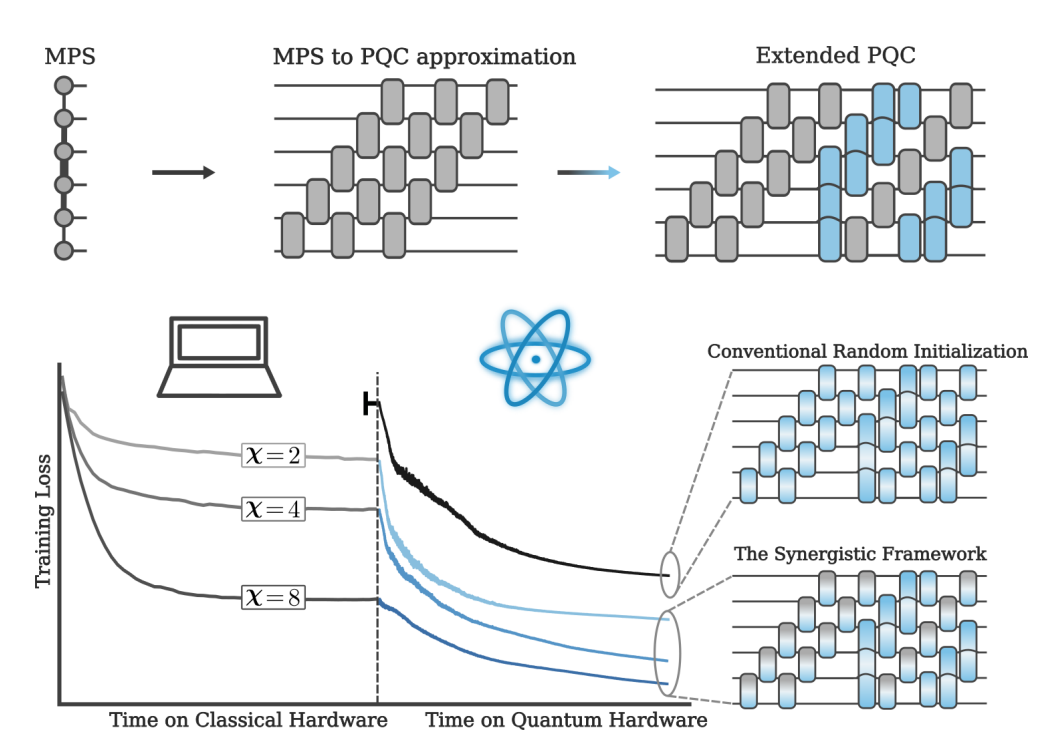
\includegraphics[scale = 0.6]{img/05-preprocesado_DMRG_VQE.png}
    \caption{Protocolo de pre-optimización DMRG-VQE}
    Fuente: adaptada de \citep{manuel}.
    \label{fig:prep_dmrg}
\end{figure}

Se puede observar como el algoritmo VQE alcanza soluciones de mejor calidad cuándo el algoritmo cuántico se inicializa con estados cuánticos provenientes de la optimización previa usando el algoritmo DMRG. Se puede observar también como la calidad de la solución del DMRG depende directamente de la dimensión interna $\chi$ del MPO utilizada, es decir, de la fidelidad entre el Hamiltoniano y el MPO creado a partir de el. Una mayor dimensión interna del MPO implica capturar una cantidad mayor de correlaciones del sistema cuántico y poder mapear a su vez un sub-espacio mayor del espacio de Hilbert, pero como contrapartida, el coste computacional crece.

\subsection{Algoritmo DMRG}
\label{sub_sec:dmrg}

El algoritmo DMRG \citep{schollwöck}, es el algoritmo de tensor  networks encargado de realizar la optimización clásica dentro de este protocolo. El algoritmo del Grupo de Renormalización de la Matriz de Densidad, o DMRG por sus siglas en inglés, tiene como objetivo encontrar el estado cuántico en forma de MPS que minimiza la energía de un operador, el Hamiltoniano problema en este caso, dado en forma de MPO. La idea es optimizar variacionalmente los tensores del MPS hasta que se cumpla un criterio de convergencia, el cual es, que se minimice la energía total del estado MPS. \\

El algoritmo DMRG trata de resolver la ecuación dada por la expresión por la expresión \ref{eq:expected_value}. No obstante, dado que lo que se busca es encontrar el estado $\ket{\psi}$ dado en forma de MPS, que minimiza la energía del Hamiltoniano dado en forma de MPO, esta expresión es computacionalmente muy costosa dado que se trata de un problema de múltiples variables desconocidas. 


\begin{equation}
    \frac{\langle \psi | H | \psi \rangle}{\langle \psi | \psi \rangle} = \lambda = E_0
    \label{eq:expected_value}
\end{equation}

Para solventar este inconveniente el algoritmo DMRG fija todo estado $\ket{\psi}$, que inicialmente se ha creado de forma aleatoria, salvo dos de los tensores, qubits, los cuales serán los que se variaran para obtener los dos tensores que localmente minimizan la energía del sistema. En la figura \ref{fig:mpo_mps} se puede observar como los tensores del MPS se han fijado salvo dos de ellos los cuales no esta definidos. El algoritmo, en este punto, calcula cuales son los dos tensores que minimiza el valor esperado de la energía.

\begin{figure}[!h]
    \centering
    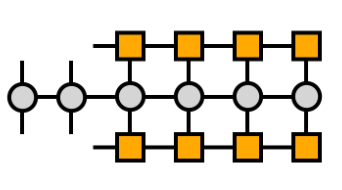
\includegraphics[scale = 0.7]{img/05-dmrg_mpo_mps.png}
    \caption{Calculo parcial del valor esperado de la energía para los primeros tensores.}
    Fuente: adaptada de \citep{tn}.
    \label{fig:mpo_mps}
\end{figure}


Una vez calculados los tensores que minimizan localmente la energía del sistema, se procede a saltar a los dos siguientes tensores del MPS tal y como se puede observar en la figura \ref{fig:mpo_mps_2}.

\begin{figure}[!h]
    \centering
    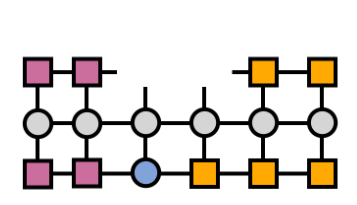
\includegraphics[scale = 0.8]{img/05-dmrg_mpo_mps_2.png}
    \caption{Calculo parcial del valor esperado de la energía para los siguientes tensores.}
    Fuente: adaptada de \citep{tn}.
    \label{fig:mpo_mps_2}
\end{figure}

Una iteración completa de optimización del algoritmo DMRG se cumple cuando se han actualizado una vez todos los tensores del MPS. Realizando una secuencia de iteraciones o \textit{sweeps} el algoritmo DMRG encontrará el estado cuántico $\ket{\psi}$, en forma de MPS, que minimiza el Hamiltoniano, en forma de MPO (ver apéndice \ref{apendix:dmrg} para mas detalles del algoritmo DMRG).

\subsection{Algoritmo de traducción MPS a PQC}
\label{sub_sec:mps_to_pqc}

El algoritmo de traducción de MPS a PQC, trata de trasladar el estado cuántico que se encuentra contenido en el MPS a un PQC. Para ello encontramos dos protocolos distintos los cuales nos permiten realizar esta tarea. Un primer protocolo, \citep{ran} utiliza una metodología analítica para traducir los estados MPS a circuitos cuánticos parametrizados. El funcionamiento del protocolo se resume en el esquema presentado en la figura \ref{fig:mps_to_pqc_a}.

\begin{figure}[!h]
    \centering
    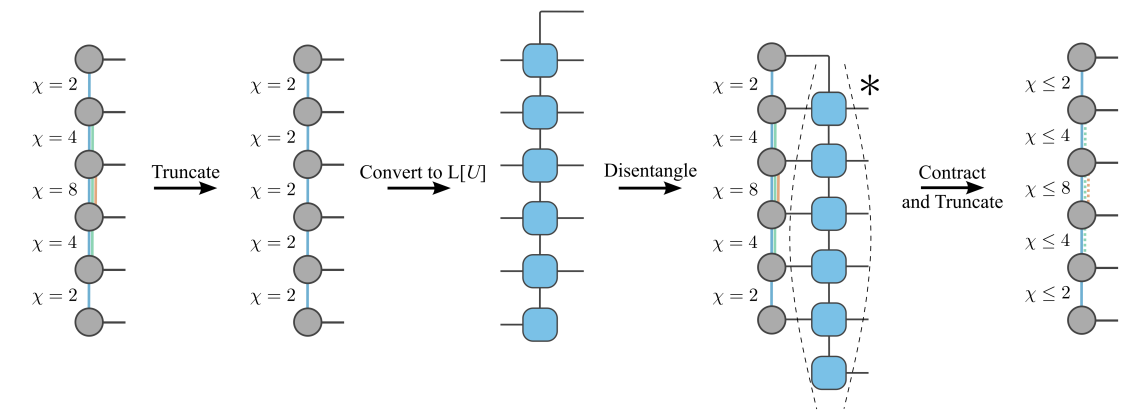
\includegraphics[scale = 0.6]{img/05-mps_to_pqc_a.png}
    \caption{Esquema de traducción analítica MPS a PQC}
    Fuente: adaptada de \citep{rudolph}.
    \label{fig:mps_to_pqc_a}
\end{figure}

\newpage

El funcionamiento base del algoritmo consiste, en un proceso iterativo que consta de varios pasos. En un primer paso se trunca el MPS inicial, que posee una dimensión máxima de $\chi = N$, a un MPS de dimensión $\chi = 2$. El segundo paso consiste en traducir el MPS de $\chi = 2$ a un producto de matrices de desentrelazamiento, o MPD por sus siglas en inglés. Este MPD se construye en base a un conjunto de reglas especificas. Esta capa de MPD construida representa la forma tensorial de las puertas cuánticas que replican en una primera aproximación el MPS de $\chi = N$, o de forma exacta al MPS de $\chi = 2$. En la figura \ref{fig:mpd_to_pqc} se observa la correspondencia entre una capa de MPD y una capa de puertas cuánticas.


\begin{figure}[!h]
    \centering
    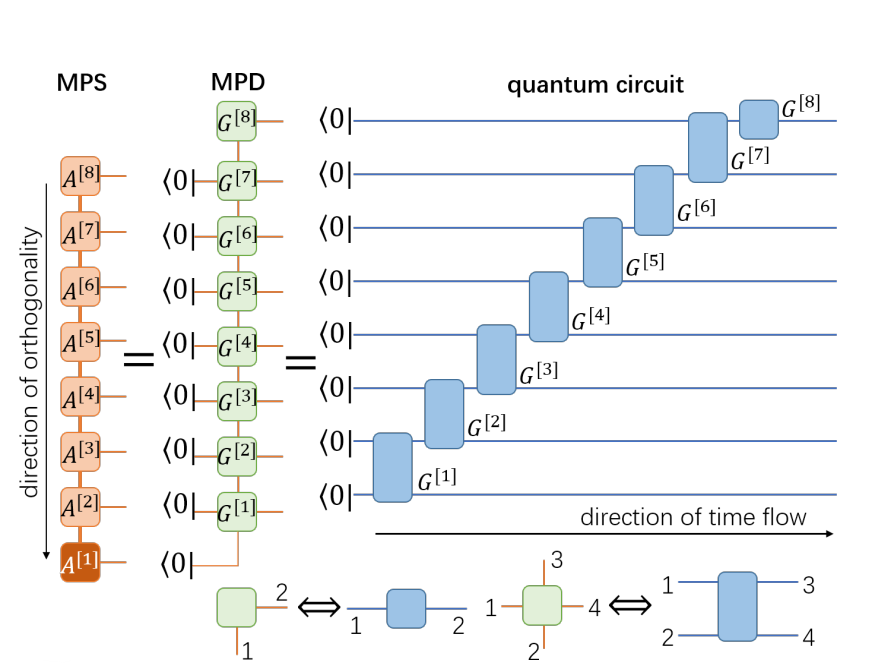
\includegraphics[scale = 0.6]{img/05-mpd_to_quantum_circuit.png}
    \caption{Traducción de MPD a PQC}
    Fuente: adaptada de \citep{ran}.
    \label{fig:mpd_to_pqc}
\end{figure}

En un tercer paso, se aplica el adjunto de la capa MPD obtenida en el paso actual sobre el estado cuántico MPS inicial. Esta operación acerca el MPS inicial a un MPS que representa el estado cuántico producto de ceros. Posteriormente se debe truncar el MPS resultante de la aplicación del MPD adjunto sobre el MPS inicial a la dimensión interna máxima de $\chi=N$. Ahora este MPS truncado actúa como el nuevo MPS inicial. Aplicando este proceso de forma iterativa obtendremos $n$ capas MPD las cuales representan $n$ capas de puertas cuánticas. El algoritmo se detiene cuando se obtiene una fidelidad entre el PQC y el MPS original o cuando se alcanzan un numero fijo de iteraciones.

\newpage

Un segundo protocolo, \citep{shirakawa}, utiliza una metodología basada en una optimización iterativa. En este segundo protocolo se propone un PQC inicial aleatorio, en forma tensorial, el cual será modificado iterativamente para que represente el estado MPS. El funcionamiento del protocolo se resume en el esquema presentado en la figura \ref{fig:mps_to_pqc_o}.


\begin{figure}[!h]
    \centering
    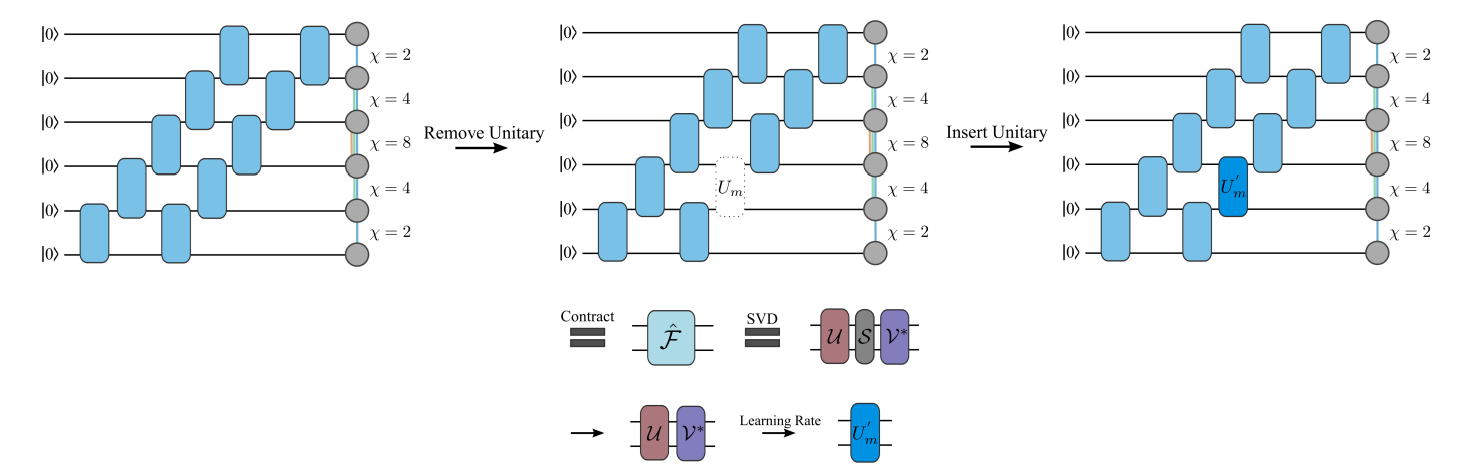
\includegraphics[scale = 0.6]{img/05-mps_to_pqc_o.png}
    \caption{Esquema de traducción por optimización MPS a PQC}
    Fuente: adaptada de \citep{rudolph}.
    \label{fig:mps_to_pqc_o}
\end{figure}

El protocolo consta de una serie de pasos que se realizan de forma iterativa. Dado un PQC propuesto inicialmente de forma aleatoria, se construye un circuito cuántico donde se encuentra inicialmente un MPS que contiene el estado cero, el PQC propuesto aplicado sobre el MPS cero y por ultimo el estado MPS que se quiere replicar. Para cada tensor de dos qubits del PQC, se calcula la expresión dada por \ref{eq:enviroment}.


\begin{equation}
    \hat{F}_m = \mathrm{Tr}_{\bar{U}_m} \left[ \prod_{i=M}^{m+1} U_i \left| \psi_{\chi_{\max}} \right\rangle \left\langle 0^{\otimes N} \right| \prod_{j=1}^{m-1} U_j^\dagger \right]
    \label{eq:enviroment}
\end{equation}

La expresión \ref{eq:enviroment} representa un nuevo tensor de dos qubits, el cual maximiza la fidelidad entre el PQC y el estado MPS objetivo. Dado que este nuevo tensor puede no ser unitario se tiene que encontrar el tensor unitario $U_{new}$ mas cercano al tensor obtenido por la expresión \ref{eq:enviroment}. Una vez encontrado el tensor $U_{new}$, unitario, se sustituye por el tensor para el cual se ha calculado la expresión \ref{eq:enviroment}. No obstante, en lugar de sustituir directamente el nuevo tensor por el antiguo dentro del PQC, se sustituye por un tensor unitario el cual es una interpolación entre el tensor nuevo y el antiguo. El tensor resultante de la interpolación se obtiene por la expresión dada por \ref{eq:interpolation}.

\begin{equation}
    U'_{m} = U_{m}(U^{\dagger}_{m}U_{new})^{r}
    \label{eq:interpolation}
\end{equation}

Donde $r$ es un coeficiente que indica el grado de interpolación, típicamente posee un valor de $r=0.6$. Una iteración del algoritmo se ha realizado, cuando se ha calculado el nuevo tensor $U'_{m}$ para cada tensor del PQC. El algoritmo se detiene cuando se ha satisfecho un criterio de convergencia o se ha alcanzado el numero de iteraciones permitidas (ver apéndice \ref{apendix:mps_to_pqc} para mas detalles de los algoritmos de traducción). \\

No obstante, las $n$ capas de puertas cuánticas de dos qubits obtenidas, ya sea usando el algoritmo analítico o el algoritmo por optimización, no pueden implementarse directamente en una QPU. Los operadores unitarios deben ser reescritos en base a un conjunto de puertas cuánticas conocidas. Para ello se realiza la llamada descomposición de Kak, \citep{tucci}. La descomposición de Kak permite traducir un operador cuántico genérico de dos qubits en terminos de puertas cuánticas parametrizadas de uno y dos qubits, tal y como puede visualizarse en \ref{fig:kak_decomposition}. Cada operador genérico de dos qubits, genera puertas cuánticas parametrizadas que contienen en total 15 parámetros. \\


\begin{figure}[!h]
    \centering
    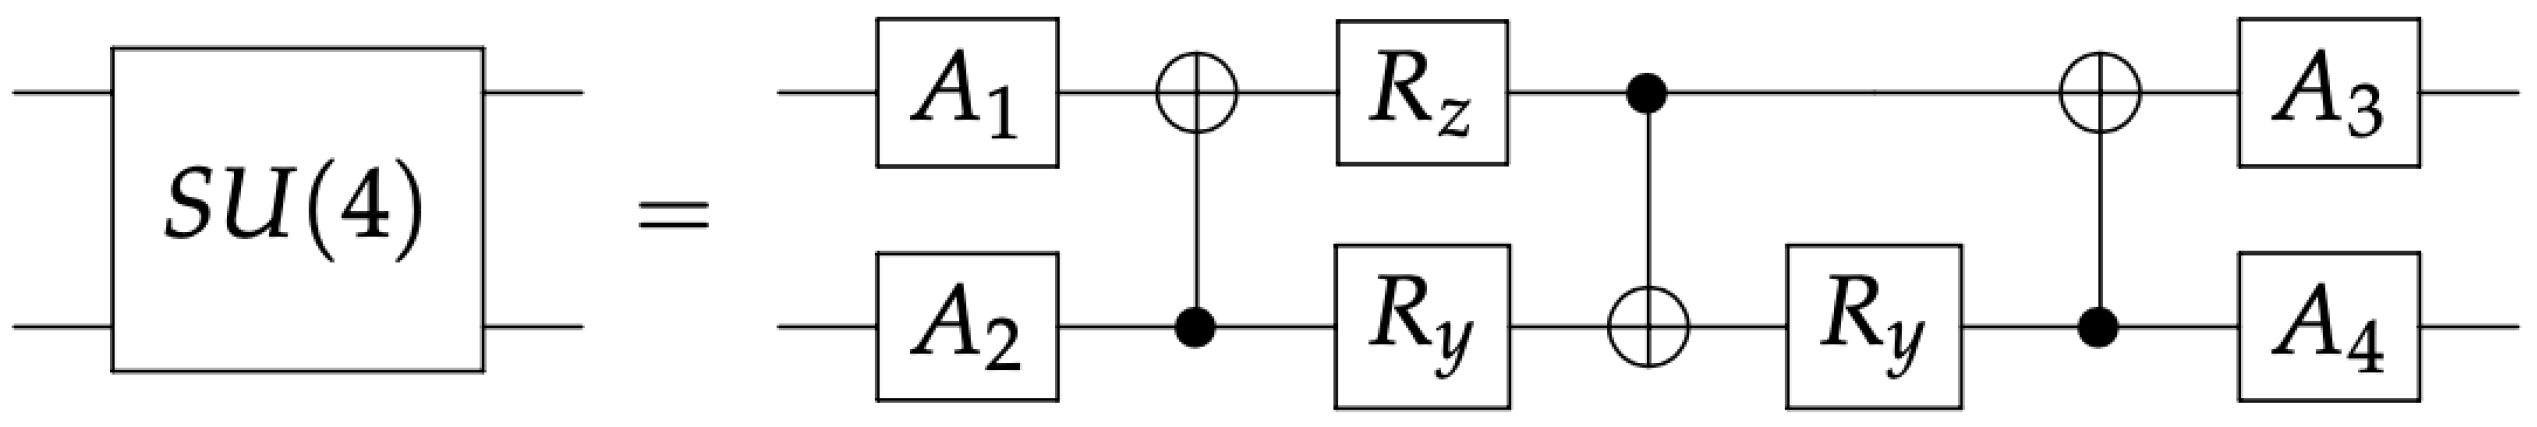
\includegraphics[scale = 0.15]{img/05-kak_decomposition.png}
    \caption{Descomposición de Kak}
    Fuente: adaptada de \citep{cenedese}.
    \label{fig:kak_decomposition}
\end{figure}

El protocolo de preprocesado DMRG implementa un algoritmo de traducción de MPS a PQC híbrido. En un primer paso se implementa un PQC inicial de $n$ capas obtenido del protocolo analítico y en un segundo paso, se optimiza, usando el algoritmo por optimización, el PQC obtenido por el algoritmo analítico. Posteriormente se añaden puertas identidad adicionales de dos qubits para aumentar la expresividad. En ultimo lugar, se aplica la descomposición de Kak para generar el circuito cuántico usado por el algoritmo VQE. \\


\newpage

\section{Protocolo de preprocesado I-TEVO}

El protocolo de preprocesado I-TEVO es un algoritmo novedoso el cual pretende ser una mejora con respecto a sus análogos del estado de la técnica. La mejora conseguida en este nuevo algoritmo de pre-optimización se basa en la hipótesis de trabajo presentada en \ref{sub_sec:hip_work}, la cual conjetura que los estados de inicialización que maximizan el rendimiento de los VQA's son los estados de Gibbs puros. \\

El protocolo I-TEVO al igual que el protocolo de pre-optimización DMRG, consta de tres partes bien diferenciadas. En un primer paso, se realiza una optimización inicial basada en la construcción de los denominados estados de Gibbs puros, mediante un algoritmo de tensor network, denominado como \textit{MPO Time Evolution}. Posteriormente estos estados de Gibbs puros, que están contenidos en MPS's, se traducen a PQC's mediante los algoritmos de traducción expuestos en el apartado \ref{sub_sec:mps_to_pqc}. Una vez se ha obtenido el PQC, que representa con alta fidelidad el estado de Gibbs puro generado, se añaden $p$ capas pertenecientes al algoritmo QAOA, con ángulos iniciales cercanos a cero. En un primer paso las capas de operadores añadidos, operador de mezcla y operador de coste, actúan como identidades, no perturbando inicialmente el estado de Gibbs puro generado, debido a sus ángulos de inicialización cercanos a cero. En un ultimo paso, se realiza la optimización por parte del algoritmo VQA's, utilizando el PQC extendido que se ha construido. \\

Es importante remarcar que, a diferencia del protocolo de preprocesado DMRG, la descomposición de Kak solo se aplica a las puertas de dos qubits generadas en el proceso de traducción de MPS a PQC. Para las capas añadidas del algoritmo QAOA, no se requiere dicha descomposición, debido a que se conoce una descomposición exacta en terminos de puertas base, \citep{jack}, cuando los Hamiltonianos problemas son de tipo Ising. Este hecho genera una ventaja sustancial en terminos del numero de parámetros que deben optimizarse, ya que cada puerta de dos qubits descompuesta mediante la descomposición de Kak genera un total de 15 parámetros. En concreto, para la implementación de este nuevo algoritmo se ha fijado la estructura de puertas provenientes del algoritmo de traducción de MPS a PQC y solo se optimizarán los parámetros contenidos en las capas de operadores añadidas. De esta manera, la parte inicial del PQC tiene como único objetivo replicar el estado de Gibbs puro, actuando así como un circuito de preparación de estado. 

\newpage

De esta forma, a diferencia del protocolo anterior, el numero de parámetros a optimizar solo depende de la profundidad del circuito y no del numero de qubits, es decir, del tamaño del problema. El esquema base del protocolo presentado se resume en la figura \ref{fig:i_tevo_qaoa}.

\begin{figure*}[htb]
\centering

\begin{tikzpicture}[scale=0.9]

    % Colors

    \filldraw[fill=classical, fill opacity=0.3, draw=black, rounded corners=5pt] (-0.5,0.5) rectangle (5,-5.5);
    %\node at (2.25, 0.8){TEVO};

    % Part 1 (left)
    \foreach \y in {0,...,4} {
        \node[circle, fill=circleColor, draw=black, minimum size=5mm] at (0, -\y) {};
        %\node[circle, fill=pastelbrown, draw=black, minimum size=5mm] at (4, -\y) {};
        \foreach \x in {1,...,4} {
            \node[rectangle, fill=orangeColor, draw=black, minimum size=5mm, rounded corners=2pt] at (\x, -\y) {};
        }
        % Horizontal connections to circles
        \draw[thick] (0.25, -\y) -- (0.75, -\y);
        \draw[thick] (3.5, -\y) -- (3.75, -\y);
        \draw[thick] (4.25, -\y) -- (4.75, -\y);
        \draw[thick] (7.75, -\y) -- (8.5, -\y);

    % Vertical connections to circles

    \foreach \y in {0,...,3}{
        \foreach \x in {0,4,7.75} {
            \draw[thick] (\x, -\y -0.25) -- (\x, -\y -0.75);
        }
    }
        
        % Connections between boxes
        \foreach \x in {1,...,3} {
            \draw[thick] (\x+0.25, -\y) -- (\x+0.75, -\y);
        }
    }
    
    % Vertical connections
    \foreach \y in {0,...,3}{
        \foreach \x in {1,...,3} {
            \draw[thick] (\x, -\y -0.25) -- (\x, -\y -0.75);
        }
    }
    
    \node at (0, -4.75) {$\ket{+}$};
    \node at (7.75, -4.75) {$\ket{\psi_{gibbs}}$};
    
    % Arrow to the middle part

    \node at (6, -2) {\huge$=$};

    \filldraw[fill=classical, fill opacity=0.3, draw=black, rounded corners=5pt] (7,0.5) rectangle (8.75,-5.5);
    
    \foreach \y in {0,...,4} {
        \node[circle, fill=pastelbrown, draw=black, minimum size=5mm] at (7.75, -\y) {};
    }

    \node at (9.15, -2) {\huge$\approx$};


    \draw[fill=tevo, draw=black, rounded corners=5pt, drop shadow] (9.5,0.5) rectangle (18,-4.5);
    
    \node at (14, 0.8){};

     \foreach \y in {0,...,4}{
        \draw[thick] (10.5, -\y) -- (17.75, -\y);
        \node at (10, -\y) {$\ket{0}$};
    }

    \foreach \x in {0,1.5, 3, 4.5}{
         \foreach \y in {0,...,3}{
             \node[rectangle, fill=pastelpurple, draw=black, minimum size=5mm, minimum width=5mm, minimum height=13mm, rounded corners=5pt] at (\y/1.6 + 10.9 +\x, -\y-0.5) {};
        }
     }
           

\end{tikzpicture}


\vspace{0.5 cm}


\begin{tikzpicture}[scale=0.9]

    % Classical box background
    \filldraw[fill=classical, fill opacity=0.3, draw=black, rounded corners=5pt] (-0.5,0.5) rectangle (4,-2.5);
    \node at (1.75, 0.8);
    
    % TEVO box
    \draw[fill=tevo, draw=black, rounded corners=5pt, drop shadow] (0,0) rectangle (3.5,-2);
    \node at (1.75, -1) {$\frac{e^{-tH}}{||e^{-tH} \ket{+}||}\ket{+}$};

    % Hybrid box background
    \filldraw[fill=hybrid, fill opacity=0.3, draw=black, rounded corners=5pt] (4.5,0.5) rectangle (16.5,-2.5);
    %\node at (10.25, 0.8) {QAOA};

    % Horizontal lines from TEVO to QAOA
    \draw (4, -0.5) -- (5, -0.5);
    \draw (4, -1) -- (5, -1);
    \draw (4, -1.5) -- (5, -1.5);

    % QAOA box 1
    \draw[fill=qaoa, draw=black, rounded corners=5pt, drop shadow] (5,0) rectangle (7,-2);
    \node at (6, -1) {$e^{-i \gamma_1 H_C}$};

    % Dotted and dashed lines inside QAOA box 1
    \draw (7, -0.5) -- (8, -0.5);
    \draw (7, -1) -- (8, -1);
    \draw (7, -1.5) -- (8, -1.5);

    % QAOA box 2
    \draw[fill=qaoa, draw=black, rounded corners=5pt, drop shadow] (8,0) rectangle (10,-2);
    \node at (9, -1) {$e^{i \alpha_1 H_M}$};

    % Dotted and dashed lines to next section
    \draw[dotted] (10, -0.5) -- (11, -0.5);
    \draw[dotted] (10, -1) -- (11, -1);
    \draw[dotted] (10, -1.5) -- (11, -1.5);

    % Repeat QAOA box 1
    \draw[fill=qaoa, draw=black, rounded corners=5pt, drop shadow] (11,0) rectangle (13,-2);
    \node at (12, -1) {$e^{-i \gamma_p H_C}$};

    % Dotted and dashed lines inside repeated QAOA box 1
    \draw (13, -0.5) -- (14, -0.5);
    \draw (13, -1) -- (14, -1);
    \draw (13, -1.5) -- (14, -1.5);

    % Repeat QAOA box 2
    \draw[fill=qaoa, draw=black, rounded corners=5pt, drop shadow] (14,0) rectangle (16,-2);
    \node at (15, -1) {$e^{i \alpha_p H_M}$};

\end{tikzpicture}

\caption{Protocolo de preprocesado I-TEVO}
Fuente: elaboración propia.
\label{fig:i_tevo_qaoa}
\end{figure*}

\subsection{Estados de Gibbs puros}

El algoritmo DMRG, tal y como se ha presentado en el apartado \ref{sub_sec:dmrg}, es un algoritmo de optimización de tensor network que trata de encontrar un estado $\ket{\psi}$ que minimiza la función de coste $f = \bra{\psi}H\ket{\psi} = E$. Sin embargo, como veremos en la sección de resultados, este criterio de búsqueda no es el mas indicado. El motivo principal reside en que el algoritmo DMRG puede encontrar estados solución con bajo o nulo grado de coherencia, esto es, grado de superposición en la base del Hamiltoniano. Se han propuesto distintas métricas para medir el grado de coherencia de un sistema cuántico. Por un lado encontramos la dimensión efectiva \citep{mori},  definida en la expresión \ref{eq:dim_efect}. 

\begin{equation}
    d_\textrm{eff}(\ket{\psi}) = \frac{1}{\textrm{Tr}\left(\ket{\psi_\textrm{d}^2}\right)}=\frac{1}{\sum_{s}|c_s|^4}
    \label{eq:dim_efect}
\end{equation}

\newpage

La dimensión efectiva da cuenta del numero de estados de la base que participan en la combinación lineal del estado $\ket{\psi}$. Por otro lado, encontramos la entropía de coherencia relativa $S_{c}(\psi||\psi_\textrm{d})$ \citep{xi}, dada por la expresión \ref{eq:s_r}.

\begin{equation}
    S_{c}(\psi||\psi_\textrm{d})=S(\rho_\textrm{d})-S(\rho) = S(\rho_\textrm{d})=S_\textrm{d}(\rho) = - \sum \eta_{i} log(\eta_{i})
    \label{eq:s_r}
\end{equation}

Donde $\rho=\sum_{i} \eta_{i} \ket{i}\bra{i}$ es matriz densidad, siendo $\ket{i}$ los autovectores de $\rho$. Para estados puros, la matriz densidad $\rho$ es idempotente y por tanto la entropía $S(\rho)$ se anula. Así, si el sistema es de dimensión finita, la entropía de coherencia relativa cuantifica la diferencia del sistema con respecto de un estado puro de la base computacional. Por tanto la entropía de coherencia, para el caso de estados puros, indica el grado de superposición de un estado cuántico, siendo un estado propio de la base del Hamiltoniano del sistema aquel que tiene entropía nula y un estado puro que es combinación lineal uniforme de todos los estados de la base, aquel que posee entropía máxima.\\

Dado que entonces el algoritmo DMRG puede arrojar estados con entropía de coherencia nula o muy baja y donde además son estados que representan mínimos locales de energía, los VQA's empezarán en mínimos de los cuales será difícil escapar. Para evitar este fenómeno, se propone una nueva función de coste, dada por la expresión \ref{eq:new_cost} en base a la cual se busquen los estados $\ket{\psi}$ usados para inicializar los VQA's. 

\begin{equation}
    f = \bra{\psi}H\ket{\psi} - \alpha S_{d}(\ket{\psi})
    \label{eq:new_cost}
\end{equation}

Donde $\alpha\geq 0$ es un hiperparametro que da cuenta de la relevancia de la entropía de coherencia, a mayor valor de $\alpha$ mayor entropía poseerá el estado cuántico. Existe un fuerte paralelismo entre la expresión \ref{eq:new_cost} y la ecuación de estado termodinámica dada por la energía libre de Gibbs dada por la expresión \ref{eq:energy_gibbs}.

\begin{equation}
    F = \bra{\psi}H\ket{\psi} - T S_{n}(\ket{\psi})
    \label{eq:energy_gibbs}
\end{equation}

Donde $S_{n}$ es la entropía termodinámica de von Neumann y $T$ la temperatura del sistema termodinámico. No obstante, la expresión \ref{eq:new_cost} es equivalente a \ref{eq:energy_gibbs}, identificando $\alpha$ como la temperatura $T$ del sistema cuántico e introducido una correspondencia directa las entropías $S_{n}$  y $S_{d}$ \citep{polkovnikov}. 

\newpage

Esta nueva función de coste, dada por la expresión \ref{eq:energy_gibbs}, es la utilizada, en este nuevo protocolo, para la inicialización de los VQA's, a diferencia de la usada por el protocolo DMRG, basaba en la expresión \ref{eq:expected_value}. Se sabe además de física estadística que los estados que minimizan la energía libre de Gibbs son aquellos estados puros que siguen la distribución Boltzman. Matemáticamente los estados que minimizan la función \ref{eq:energy_gibbs} y que denominamos estados de Gibbs puros, se definen por la expresión \ref{eq:gibbs_states}.

\begin{equation}
    \ket{\psi(\beta)}=\frac{1}{\sqrt{Z_\beta}}\sum_s e^{-\beta E(s)/2} e^{i\theta_s}\ket{s}
    \label{eq:gibbs_states}
\end{equation}

Donde $\beta=1/T$ es la inversa de la temperatura, 
$Z_\beta=\sum_{s} e^{-\beta E(s)}$ es la función de partición del Hamiltoniano y
$\theta_s$ es un conjunto de fases arbitrarias que por simplicidad les datemos el valor de $\theta_s=0$ para todo $s$.

\subsection{Diagrama entropía-energía}

Los estados de Gibbs puros son extrémales, pues dado un nivel de energía, los estados de Gibbs puros son aquellos que maximizan la entropía. Por el contrario, dado un nivel de entropía, los estados de Gibbs puros son aquellos que minimizan la energía del sistema. En este punto es útil introducir el denominado diagrama de \textit{energía-entropía}, usado en artículos de la literatura academia relativa a la trabajos de termodinámica \citep{riera}. Dado un sistema descrito por un Hamiltoniano $H$, un estado $\psi$ del sistema se representa dentro del diagrama entropía-energía por un punto con coordenadas $x(\psi) = (E(\psi), S_{d}(\psi))$ tal y como se muestra en la figura \ref{fig:energy-entropy-diagram}.


\begin{figure*}[h]
\begin{center}
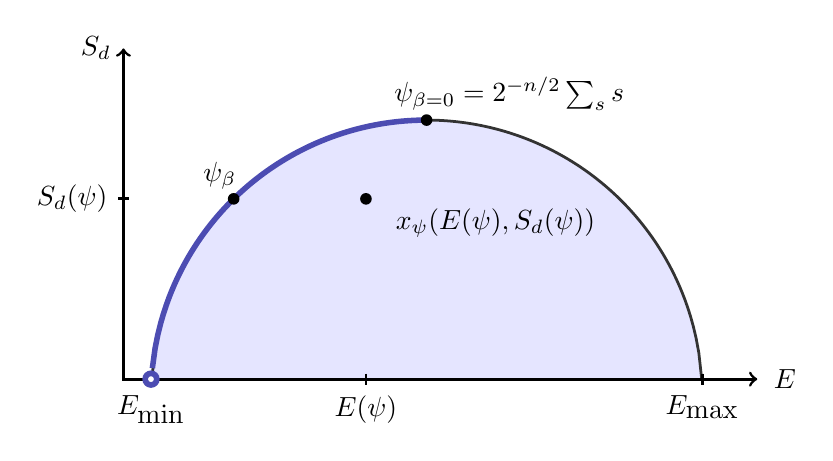
\begin{tikzpicture}[scale=3.5,
declare function={
        func(\x) = sqrt(\x*(2-\x))-0.06;
      }]

\begin{scope}
\clip (-0.1,1.2) rectangle (2.2,0);
\draw[black!80!white, line width=1pt, domain=0:2,fill=blue!10!white, samples=200]  plot (\x,{func(\x)});
\end{scope}
\draw[gray!60!blue, line width=2pt, domain=0.005:1, samples=100]  plot (\x,{func(\x)});

\draw [<->, line width=1pt] (-0.1,1.2) -- (-0.1,0) -- (2.2,0);
\node[] at (-0.2,1.2) { $S_d$};
\node[] at (2.3,0) { $E$};
 
% free and bound energy
\fill (1.,{func(1)}) circle (.6pt);
\node[above] at (1.3,{func(1)}) { $\ket{\psi_{\beta=0}}=2^{-n/2}\sum_s\ket{s}$};
\fill (.3,{func(.3)}) circle (.6pt);
\node[above] at (.25,{func(.3)}) {$\ket{\psi_\beta}$};
\fill (.78,{func(.3)}) circle (.6pt);
\node[below] at (1.25,{func(.3)}) {$x_\psi\coloneqq(E(\psi),S_d(\psi))$};
\draw [line width=1pt] (0.78,.02) -- (.78,-.02) node[below] {$E(\psi)$};
\draw [line width=1pt] (2,.02) -- (2,-.02) node[below] {$E_{\textrm{max}}$};
\draw [line width=1pt] (0.0,.02) -- (0,-.02) node[below] {$E_{\textrm{min}}$};
\fill [color=gray!60!blue](0,0) circle (.9pt);
\fill [color=white](0,0) circle (.3pt);


\draw [line width=1pt] (-0.08,{func(.3)}) -- (-.12,{func(.3)}) node[left] {$S_d(\psi)$};
\end{tikzpicture}

\caption{Diagrama entropía-energía}
Fuente: elaboración propia.
\label{fig:energy-entropy-diagram}
\end{center}
\end{figure*}

En este trabajo introducimos el diagrama entropía-energía con la entropía diagonal y lo restringimos a estados puros. Así, todos los estados puros residen en una región que está limitada inferiormente por el eje horizontal, es decir $S_d=0$,  correspondiente a los autoestados del Hamiltoniano, y limitada superiormente por la curva convexa $(E(\beta),S(\beta))$, 
que representa los estados puros de Boltzmann de temperaturas positivas y negativas. Denotemos tal curva como el \emph{límite de Boltzmann}. Además, la inversa de la temperatura asociada a un punto de la frontera de Boltzmann viene dada por la pendiente de la recta tangente en dicho punto, es decir por la expresión \ref{eq:temperature}.

\begin{equation}
  \beta = \frac{d S(\beta)}{d E(\beta)}
  \label{eq:temperature}
\end{equation}

Dentro de este diagrama el estado de superposición uniforme, también denominado como estado Hadamard, es un caso particular de estado de Gibbs puro, el cual posee una temperatura positiva infinita. De igual forma, el estado fundamental del Hamiltoniano, aquel que posee energía mínima, esta asociado a un estado de Gibbs de temperatura cero. A medida que los estados de Gibbs disminuyen su temperatura 

\subsection{Algoritmo MPO Time Evolution}

El algoritmo MPO Time Evolution \citep{zaletel}, es el algoritmo de tensor networks encargado de la creación de los estados de Gibbs puros, que serán utilizados en la inicialización de los VQA's.\\

MPO Time Evolution implementa una aproximación del operador $e^{- i t H}$, es decir, el operador evolución temporal para un Hamiltoniano independiente del tiempo. Si se denota, $i t$ como $\tau$, entonces el operador que implementa MPO Time Evolution es $e^{- \tau H}$ el cual es una evolución temporal imaginaria del sistema cuántico. La decisión de utilizar MPO Time Evolution para representar la evolución imaginaria del sistema cuántico reside en principalmente en dos aspectos. En primer lugar, el error introducido en la aproximación es independiente del tamaño del sistema, esto es importante, ya que garantiza el poder utilizar esta metodología para tamaños de problemas arbitrariamente grandes, manteniendo un error constante. En segundo lugar, esta metodología permite implementar la evolución temporal, real o imaginaria, de Hamiltonianos que poseen interacciones no locales. Esto es importante, dado que los problemas de nuestro interés, como el problema Max Cut, son problemas cuyos Hamiltonianos típicamente poseen interacciones no locales. 

\newpage

Sea un Hamiltoniano de la forma $H = \sum_{x} H_{x}$, un Hamiltoniano que puede expresarse como suma de terminos individuales. Este Hamiltoniano puede reescribirse tal y como se muestra en la expresión \ref{eq:hamiltonian}.

\begin{equation}
  H = H_{L_i} \otimes \mathbb{I}_{R_i} + \mathbb{I}_{L_i} \otimes H_{R_i} + \sum_{a_i=1}^{N_i} h_{L_i, a_i} \otimes h_{R_i, a_i}
  \label{eq:hamiltonian}
\end{equation}

Donde $H_{L_i}/H_{R_i}$
son las componentes del Hamiltoniano localizados a la izquierda y a la derecha del enlace en el que nos situamos, dado que trabajamos en sistemas 1D, mientras que $h_{L_i, a_i} \otimes h_{R_i, a_i}$ son los terminos de interacción que atraviesan el enlace. Existe una recursión entre las descomposiciones en enlace (i-1, i) y (i, i + 1), que se diferencian por la adición del sitio i tal y como se puede observar en la expresión \ref{eq:mpo_h}.

\begin{equation}
  \begin{pmatrix}
H_{R_{i-1}} \\
h_{R_{i-1}, a_{i-1}} \\
\mathbb{I}_{R_{i-1}}
\end{pmatrix}
=
N_{i-1}
\begin{pmatrix}
\hat{\mathbb{I}} & \hat{C} & \hat{D} \\
0 & \hat{A} & \hat{B} \\
0 & 0 & \hat{\mathbb{I}}
\end{pmatrix}_{(i)}
\otimes
\begin{pmatrix}
H_{R_i} \\
h_{R_i, a_i} \\
\mathbb{I}_{R_i}
\end{pmatrix}
\label{eq:mpo_h}
\end{equation}

La matriz central de \ref{eq:mpo_h} representa el operador del MPO para la posición $i-esima$ que representa al Hamiltoniano descrito en \ref{eq:hamiltonian}. Dado el tensor $i-esimo$ del MPO, el algoritmo MPO Time Evolution implementa la aproximación en primer y segundo orden del desarrollo en serie de Taylor del operador evolución temporal $U(t) = e^{-it H}$ . Sea \ref{eq:taylor}, el desarrollo de Taylor del operador $U(t)$.


\begin{equation}
U(t) = 1 + t \sum_{x} H_x + \frac{1}{2} t^2 \sum_{x,y} H_x H_y + \ldots
\label{eq:taylor}
\end{equation}

La expresión \ref{eq:taylor} no tiene una representación eficiente en MPO para poder implementar un paso de tiempo de Euler de la forma $\prod_{x}(1 + t H_{x})$. No obstante, el desarrollo de Taylor modificado, dada por la expresión \ref{eq:taylor_1} si posee una representación trivial en MPO.

\begin{equation}
U^I(t) = 1 + t \sum_{x} H_x + t^2 \sum_{x<y} H_x H_y + t^3 \sum_{x<y<z} H_x H_y H_z + \ldots
\label{eq:taylor_1}
\end{equation}

Donde se denota $x<y$ como los terminos de $H_x$ que se encuentran estrictamente a la izquierda del sitio afectado por $H_y$. 

\newpage

Para la expresión \ref{eq:taylor_1} el MPO que implementa un paso de tiempo de Euler de la forma $\prod_{x}(1 + t H_{x})$, viene dada por la expresión \ref{eq:mpo_tevo}


\begin{equation}
W^{I}_{(i)}(t) =
\begin{pmatrix}
\hat{\mathbb{I}_{(i)}} + t \hat{D_{(i)}} & \sqrt{t}\hat{C_{(i)}} \\
 \sqrt{t}\hat{B_{(i)}} & \hat{A_{(i)}} 
\end{pmatrix}_{(i)}
\label{eq:mpo_tevo}
\end{equation}

Cada tensor del MPO que implementa la aproximación en primer orden del operado $U(t)$ se construye trivialmente a partir del MPO dado por la expresión \ref{eq:mpo_h}. 

\subsection{Construcción de estados de Gibbs puros}

Una vez, se ha construido el MPO que representa $U^{I}(t)$, se pueden construir los estados de Gibbs puros. Para ello, usaremos la evolución imaginaria, es decir la evolución dada por el operador $U = e^{- \tau H}$. Los estados de Gibbs puros, tomando el conjunto de fases con valor cero y agrupando constantes, vienen dados por la expresión \ref{eq:gibbs_states_simpli}.

\begin{equation}
    \ket{\psi(\beta)}=\frac{1}{\sqrt{\sum_s e^{-\beta E(s)}}}\sum_s e^{- \beta E(s)}\ket{s}
    \label{eq:gibbs_states_simpli}
\end{equation}

Los estados de Gibbs dados por \ref{eq:gibbs_states_simpli}, pueden construirse mediante la aplicación del operador $U = e^{- \tau H}$, en forma de MPO, aplicado sobre el estado $\ket{\psi(\beta=0)}$, en forma de MPS, tal y como se puede observar en la expresión \ref{eq:gibbs_states_tevo}.

\begin{equation}
\ket{\psi_\beta}= \frac{e^{-\beta H_P}\ket{\psi_{\beta=0}}}{|| e^{-\beta H_P}\ket{\psi_{\beta=0}}||}   
\label{eq:gibbs_states_tevo}
\end{equation}

Sin embargo, algoritmo MPO Time Evolution solo nos permite implementar un paso de tiempo $\delta \tau$. Para poder realizar una evolución imaginaria de tiempo total $t$, es necesario aplicar $p$ capas de $U^{I}$ los cuales evolucionen el sistema un tiempo $p \cdot \delta \tau$. La relación entre la temperatura del estado de Gibbs generado y el tiempo de evolución imaginario implementado viene dada por la relación \ref{eq:time_temperature}.

\begin{equation}
\beta = t = \frac{1}{T} 
\label{eq:time_temperature}
\end{equation}

De esta forma, evolucionar durante un tiempo imaginario total $t$ el sistema cuántico, implica alcanzar un estado de Gibbs puro de temperatura $T=\frac{1}{t}$.

\newpage

La construcción de los estados de Gibbs puros en base al algoritmo MPO Time Evolution viene dado de forma esquemática por la figura \ref{fig:mpo_time_evolution}. El sistema comienza en el estado $\ket{\psi(\beta = 0)}$, el cual es equivalente al estado Hadamard o de superposición uniforme. Seguidamente se aplican $p$ capas de MPO's los cuales son la representación aproximada de la expresión \ref{eq:taylor_1}. Cada capa de MPO hace evolucionar al sistema un tiempo imaginario $\delta \tau$. Después de la aplicación de cada capa de MPO es necesario realizar un proceso de truncación sobre el estado MPS resultante para evitar que la dimensión interna del MPS crezca de forma desproporcionada. 

\begin{figure}[!h]
    \centering
    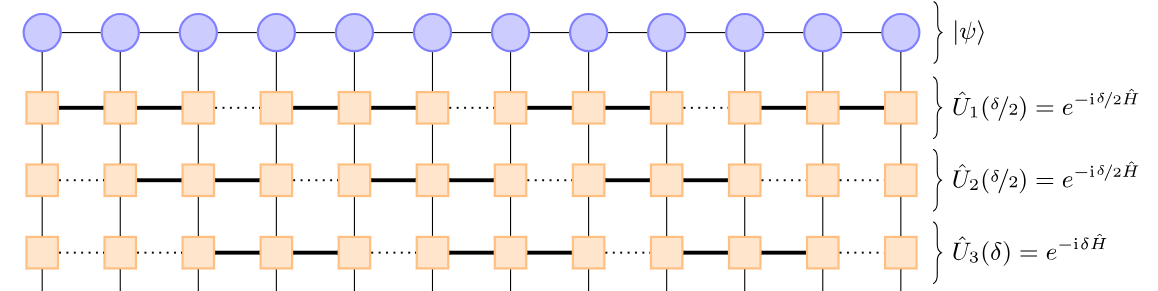
\includegraphics[scale = 0.7]{img/05-tevo_mps_mpo.png}
    \caption{Algoritmo MPO Time Evolution}
    Fuente: adaptada de \citep{tn}.
    \label{fig:mpo_time_evolution}
\end{figure}

El proceso de truncación a cada paso, introduce un error adicional al proceso, el cual posee dos fuentes principales de error. Una primer fuente de error proviene de la aproximación en primer orden del operador dada por \ref{eq:taylor_1}, el cual posee un error de $(\delta \tau)^2$. Por otro lado, el error proveniente del proceso de truncación del MPS. Estos dos fuentes de error limitan el tiempo total durante el cual el sistema cuántico puede ser evolucionado. Después del proceso de aplicación y truncación de las $p$ capas de MPO's, se obtendrá el MPS que representa el estado de Gibbs a temperatura $T = \frac{1}{t}$ (ver apéndice \ref{apendix:mpo_time_evolution} para mas detalles del algoritmo MPO Time Evolution).
\chapter{Discusión de resultados}
\label{chapter:results}

En este capítulo se presentan todos los resultados numéricos obtenidos de las simulaciones llevadas a cabo. El objetivo de las siguientes gráficas que se van a presentar dentro de este capítulo son dos. En primer lugar validar la hipótesis presentada en el apartado \ref{sub_sec:hip_work}, la cual es el punto central del algoritmo de pre-optimización novedoso desarrollado en este documento. En segundo lugar, realizar una comparativa entre los dos métodos de pre-optimización implementados en este proyecto, siendo el primero, perteneciente al estado de la técnica y el segundo, un método novedoso. El problema utilizado y con el cual se han llevado a cabo todas las simulaciones, es el presentado en el apartado \ref{sub:problem_target}.

\section{Inicialización con estados de Gibbs puros}
\label{sub_sec:result_gibbs_states}

Con el objetivo de demostrar numéricamente que los estados de Gibbs puros maximizan el rendimiento del algoritmo QAOA, vamos a utilizar como apoyo el diagrama entropía-energía. Tomando el diagrama entropía-energía, dada por la Figura \ref{fig:energy-entropy-diagram-mod}, para cualquier estado de Gibbs puro situado en el límite de Boltzmann y representado por el punto azul, se quiere comparar con los estados situados en los puntos rojo y marrón, así como los situados a los largo de las lineas naranja y verde.


\begin{figure*}[h]
\begin{center}
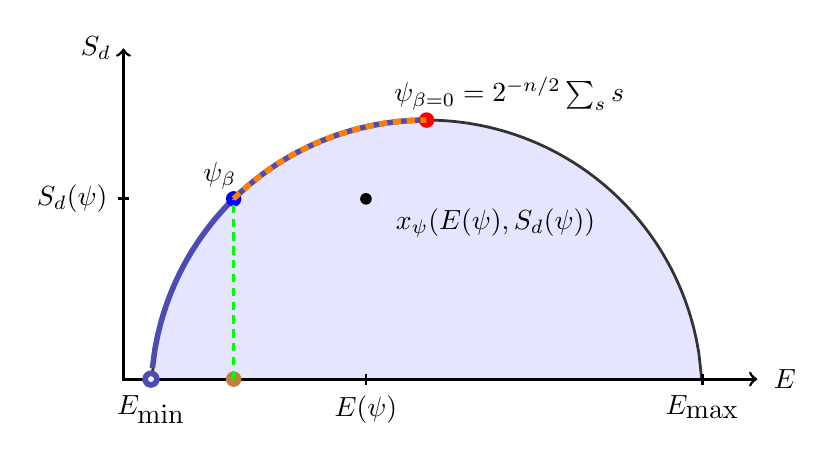
\begin{tikzpicture}[scale=3.5,
declare function={
        func(\x) = sqrt(\x*(2-\x))-0.06;
      }]

\begin{scope}
\clip (-0.1,1.2) rectangle (2.2,0);
\draw[black!80!white, line width=1pt, domain=0:2,fill=blue!10!white, samples=200]  plot (\x,{func(\x)});
\end{scope}
\draw[gray!60!blue, line width=2pt, domain=0.005:1, samples=100]  plot (\x,{func(\x)});

\draw [<->, line width=1pt] (-0.1,1.2) -- (-0.1,0) -- (2.2,0);
\node[] at (-0.2,1.2) { $S_d$};
\node[] at (2.3,0) { $E$};
 
% free and bound energy
\fill (1.,{func(1)}) circle (.6pt);
\node[above] at (1.3,{func(1)}) { $\ket{\psi_{\beta=0}}=2^{-n/2}\sum_s\ket{s}$};
\fill (.3,{func(.3)}) circle (.6pt);
\node[above] at (.25,{func(.3)}) {$\ket{\psi_\beta}$};
\fill (.78,{func(.3)}) circle (.6pt);
\node[below] at (1.25,{func(.3)}) {$x_\psi\coloneqq(E(\psi),S_d(\psi))$};
\draw [line width=1pt] (0.78,.02) -- (.78,-.02) node[below] {$E(\psi)$};
\draw [line width=1pt] (2,.02) -- (2,-.02) node[below] {$E_{\textrm{max}}$};
\draw [line width=1pt] (0.0,.02) -- (0,-.02) node[below] {$E_{\textrm{min}}$};
\fill [color=gray!60!blue](0,0) circle (.9pt);
\fill [color=white](0,0) circle (.3pt);

\fill [color=blue](0.3,{func(.3)}) circle (0.8pt);
\fill [color=red](1,{func(1)}) circle (0.8pt);
\fill [color=brown](0.3,0) circle (.8pt);

\draw [green, densely dashed, line width=1pt] (0.3,0) -- (0.3,{func(.3)});

\draw[orange, densely dashed, line width=2pt, domain=0.3:1, samples=100]  plot (\x,{func(\x)});

\draw [line width=1pt] (-0.08,{func(.3)}) -- (-.12,{func(.3)}) node[left] {$S_d(\psi)$};
\end{tikzpicture}

\caption{estados de interés en el diagrama entropía-energía}
\label{fig:energy-entropy-diagram-mod}
\end{center}
\end{figure*}

De esta forma comparamos los estados de Gibbs a una temperatura dada, energía y entropía fija, con los estados que comparten características similares pero no exactamente iguales.

\newpage

Los estados situados a lo largo de la linea verde, incluido el punto marrón, poseen la misma energía que el estado de Gibbs, representado por el punto azul, pero menor entropía. Por otro lado, los estados de Gibbs, situados a los largo de la linea naranja incluido el punto rojo, poseen mayor entropía que el estado de Gibbs pero también mayor energía. Para comparar la calidad de la solución obtenida por el algoritmo QAOA inicializado con el estado correspondiente, se usará la diferencia de energía relativa denotada por $\alpha$. La diferencia de energía relativa viene dado por la expresión \ref{eq:diference_relative}. Un valor positivo de $\alpha_{r}(x,y)$ implicaría que la calidad de la solución de $y$ es mayor que la de $x$, dado que la calidad de energía relativa $\alpha$ es máxima cuando toma el valor cero.

\begin{equation}
    \alpha_{r}(x, y) = \alpha(x) - \alpha(y) = \frac{|E_{exacta}| - |E_{x}|}{|E_{exacta}|} - \frac{|E_{exacta}| - |E_{y}|}{|E_{exacta}|}
    \label{eq:diference_relative}
\end{equation}

En primer lugar, presentamos el gráfico dado por la Figura \ref{fig:gibbs_product}, la cual compara estados de Gibbs, punto azul, con estados producto, punto marrón.

\begin{figure}[!h]
    \centering
    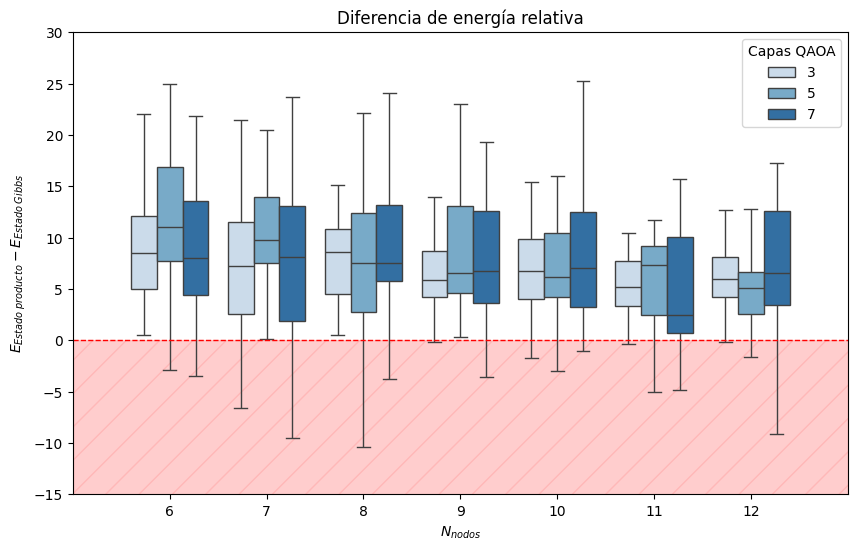
\includegraphics[scale = 0.7]{plt/06-gibbs_vs_producto.png}
    \caption{diferencia relativa de energía entre estados de Gibbs y estados producto a $T=4$}
    \label{fig:gibbs_product}
\end{figure}

En la Figura \ref{fig:gibbs_product} se muestra como varía $\alpha_{r}$(estado producto, estado Gibbs) con el tamaño del problema. \\ 

Se puede observar que de forma consistente, independientemente del tamaño del problema o del numero de capas del algoritmo QAOA, la calidad de la solución obtenida por el algoritmo es mejor cuando este se inicializa con estados de Gibbs en lugar de estados producto que poseen la misma energía de partida. Cada diagrama de caja del gráfico es el resultado de 30 simulaciones, lo que da un total de 540 simulaciones llevadas a cabo para la generación del gráfico. \\

La siguiente gráfica presentada, dada por la Figura \ref{fig:gibbs_hadamard_nodes} compara estados de Gibbs,  punto azul, con el estado Hadamard, punto rojo, a una temperatura fija de $T=4$, es decir se presenta $\alpha_{r}$(estado Hadamard, estado Gibbs). 

\begin{figure}[!h]
    \centering
    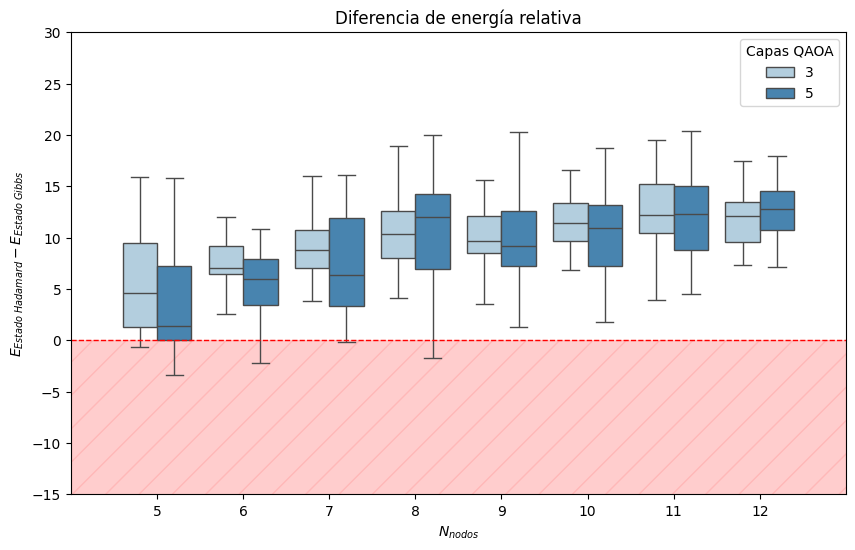
\includegraphics[scale = 0.7]{plt/06-gibbs_vs_hadamard_nodes.png}
    \caption{diferencia relativa de energía entre estados de Gibbs y el estado Hadamard a $T=4$}
    \label{fig:gibbs_hadamard_nodes}
\end{figure}

Al igual que con la Figura \ref{fig:gibbs_product}, el algoritmo QAOA, inicializado con estados de Gibbs a temperatura $T=4$, arroja un rendimiento superior, independientemente del numero de capas. 

\newpage

Se puede observar como un aumento del tamaño del problema genera una mayor distancia entre la calidad de la solución obtenida por el QAOA inicializado con el estado Hadamard y el QAOA inicializado por el estado de Gibbs. Este hecho se produce debido a que la energía de partida del estado Hadamard es creciente con el tamaño del problema, dado que es un promedio energético de todas las soluciones posibles del problema. De igual forma, cada diagrama de caja ha sido el resultado de 30 simulaciones, lo que da un total de 420 simulaciones llevadas a cabo para la generación del gráfico. \\


La siguiente gráfica que se presenta, es también una comparación entre estados de Gibbs y estados Hadamard, pero ahora a un tamaño de problema fijo, en el cual se varia la temperatura. Lo que se va a comparar es como varia $\alpha_{r}(estado \; Hadamard, estado \; Gibbs)$ cuando nos desplazamos a lo largo de la linea naranja del diagrama \ref{fig:energy-entropy-diagram-mod}. En la Figura \ref{fig:gibbs_hadamard_temperature} se presenta dicha comparación para un problema de tamaño $N=16$.

\begin{figure}[!h]
    \centering
    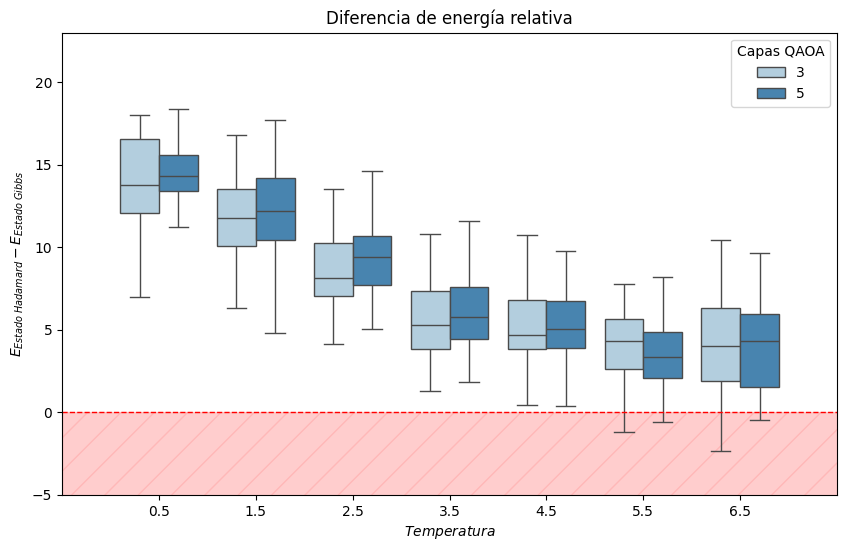
\includegraphics[scale = 0.75]{plt/06-gibbs_vs_hadamard_temperature.png}
    \caption{diferencia relativa de energía entre estados de Gibbs y el estado Hadamard con $N=16$}
    \label{fig:gibbs_hadamard_temperature}
\end{figure}

\newpage

Se puede observar en la Figura \ref{fig:gibbs_hadamard_temperature} como a medida que nos desplazamos a lo largo de la linea naranja, lo cual es equivalente a estados de Gibbs de menor temperatura, tal como marca la relación \ref{eq:time_temperature}, la diferencia de calidad entre el estado Hadamard y el estado de Gibbs especifico aumenta. Además podemos observar que la función es monótona creciente dado que una reducción en la temperatura implica necesariamente una mejora en la calidad de la solución obtenida por el QAOA.  De igual forma, cada diagrama de caja ha sido el resultado de 30 simulaciones, lo que da un total de 420 simulaciones llevadas a cabo para la generación del gráfico. \\

Las Figuras \ref{fig:gibbs_hadamard_nodes} y \ref{fig:gibbs_hadamard_temperature} son además de especial utilidad para mostrar la potencia de los estados de Gibbs puros. En numerosos artículos del estado de la técnica, como el trabajo de \cite{shaydulin}, muestran numéricamente que para el algoritmo QAOA, los estados que maximizan el rendimiento del algoritmo son los estados fundamentales del Hamiltoniano de mezcla, que para el caso del QAOA genérico, es el estado Hadamard. No obstante aquí se comprueba que existen otros estados no triviales, que consiguen un rendimiento del QAOA consistentemente mejor que el estado Hadamard. \\

Por último, queda comparar los estados de Gibbs con aquellos estados que poseen una misma energía pero distinta entropía no nula, es decir aquellos estados situados a lo largo de la linea verde del diagrama \ref{fig:energy-entropy-diagram-mod}. Tal y como se puede observar en la gráfica \ref{fig:entropia_vs_energia_pseudogibbs}, dado un conjunto de estados donde todos ellos poseen la misma energía, pero distinta entropía, aquellos que maximizan el rendimiento del algoritmo QAOA son aquellos que poseen entropía de coherencia máxima. La normalización de la entropía asociada a cada estado se realiza en base a la entropía del estado de Gibbs en ese punto, dado que a una energía determinada, dicho estado maximiza la entropía. Es claro, que a medida que nos acercamos al limite del Boltzmann, es decir, aumentamos la entropía del estado de inicialización, la calidad de la solución arrojada por el algoritmo QAOA, en forma de energía relativa con respecto a la solución exacta, aumenta de forma consistente. \\

La metodología llevada a cabo para la construcción de estados de \textit{pseudoGibbs}, es decir estados cercanos al limite del Boltzmann, ha sido mediante la creación de estados gaussianos. Dado un estado de Gibbs a temperatura $T$, dicho estado posee una energía fija $E_{T}$.


\newpage

\begin{figure}[!h]
    \centering
    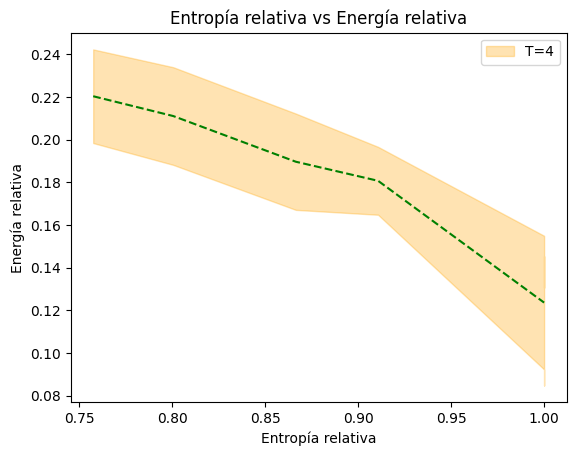
\includegraphics[scale = 0.75]{plt/06-entropia_vs_energia_pesudo_gibbs.png}
    \caption{calidad de la solución obtenida en función de la entropía del estado de pseudoGibbs para tamaños de $N=9$}
    \label{fig:entropia_vs_energia_pseudogibbs}
\end{figure}

Para construir estados gaussianos que representan estados de pseudoGibbs utilizamos la expresión dada por \ref{eq:psgibbs_state}.

\begin{equation}
    \ket{\psi_{\text{psGibbs}}(E_{T})} = \frac{1}{\sigma \sqrt{2 \pi}} \sum_{i}e^{-\frac{(E_{i} - E_{T})^2}{2 \sigma^2}} \ket{i}
    \label{eq:psgibbs_state}
\end{equation}

Donde $\ket{i}$ son los estados propios del Hamiltoniano, $E_{i}$ es el valor propio de la energía asociado al estado $\ket{i}$, $E_T$ es el valor en el cual se centra la gaussiana y donde $\sigma$ es la desviación estandar de la gaussiana, es decir la anchura de la distribución normal. Mediante el parámetro $\sigma$ podemos controlar la cantidad de estados que participan en la combinación lineal del estado de pseudoGibbs que posee energía $E_T$, es decir que podemos controlar la entropía del estado. Un valor de $\sigma$ mas alto, implica una mayor cantidad de estados que participan de la combinación lineal, aumentando así la entropía. \\

A traves de esta metodología, hemos podido validar numéricamente la hipotesis presentada en el apartado \ref{sub_sec:hip_work} para el caso del algoritmo variacional QAOA. Una forma alternativa de visualizar los resultados presentados que es mas intuitiva y descriptiva, aunque solo es el resultado de un caso particular, aunque aleatorio, es mediante un mapa de calor. 

\newpage

Usando el diagrama de entropía-energía podemos representar la calidad de los resultados obtenidos por el algoritmo QAOA en función de estados de inicialización y ordenarlos según el propio diagrama entropía-energía. En la Figura \ref{fig:mapa_calor} puede observarse el mapa de calor de un problema concreto de Max Cut de 10 nodos para un QAOA de 3 capas.


\begin{figure}[!h]
    \centering
    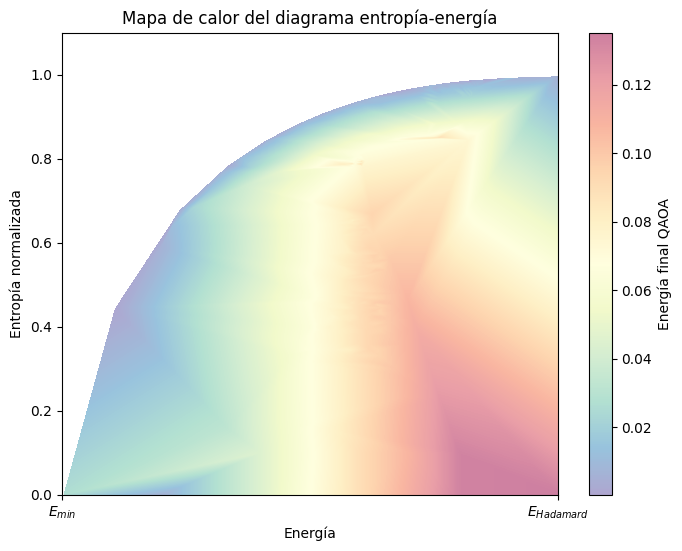
\includegraphics[scale = 0.8]{plt/06-mapa_calor.png}
    \caption{mapa de calor del algoritmo QAOA de tres capas para un problema de $N=8$}
    \label{fig:mapa_calor}
\end{figure}

Se puede observar que según el mapa de calor presentado, los estados que maximizan el rendimiento del algoritmo QAOA, aquellos estados que de inicialización que maximizan la calidad de la solución obtenida por QAOA, son los estados del limite de Boltzmann. Por otro lado, los estados situados en el núcleo del diagrama son aquellos que peor rendimiento arrojan como estados de inicialización (ver apéndice \ref{apendix:energy_landscape}  para más detalle). Para evitar que aquellos estados que ya se encuentran cerca del mínimo arrojen soluciones mejores solo por el hecho de encontrarse cerca del estado exacto, la energía final del QAOA presentada como código de colores dentro de la figura \ref{fig:mapa_calor}, se normaliza con respecto a la energía final del QAOA obtenida por los estados de Gibbs en cada punto.

\newpage

De esta forma, la calidad de la solución se compara siempre con respecto a los estados de Gibbs, y tal como puede observarse, no hay ningún estado dentro del diagrama que mejore la solución obtenida por los estados de Gibbs.

\section{Protocolos de pre-optimización}

Habiendo mostrado evidencias numéricas de que los estados de Gibbs puros, situados en el limite de Boltzmann maximizan el rendimiento del algoritmo QAOA, podemos aseverar que el protocolo mostrado en la sección \ref{sub_sec:dmrg} arrojará un rendimiento peor que el protocolo novedoso presentado en la sección \ref{sub_sec:i_tevo}. No obstante es difícil comparar justamente ambos protocolos dado que son bastante diferente entre ellos. El algoritmo de tensor networks de pre-optimización es totalmente distinto, usando el primer protocolo el algoritmo DMRG y el segundo, el algoritmo MPO Time Evolution. Además, los \mbox{PQC} utilizados también difieren, ya que el primero utiliza un conjunto de puertas cuánticas de dos qubits $SU(4)$ con una cantidad de parámetros a optimizar, creciente con el tamaño del problema, mientras que el segundo utiliza un \mbox{PQC} fijo para la preparación del estado de inicialización con un conjunto de capas de QAOA añadidas para ser optimizadas. \\

No obstante podemos presentar un conjunto de gráficas, que muestran el rendimiento dispar que poseen ambos protocolos de pre-optimización cuando se pretende resolver un problema clásico como el Max Cut. En la Figura \ref{fig:comparativa_protocolo} comparamos ambos métodos de pre-optimización para resolver un problema concreto de Max Cut de un grafo de $N=10$. Se puede observar que, aunque el algoritmo DMRG del primer protocolo converge mas rápido a un estado de menor energía posteriormente, el algoritmo VQE es incapaz de  mejorar el resultado de partida dado por el algoritmo DMRG. El motivo de esto, se debe a que el algoritmo DMRG a convergido a un estado de baja energía pero también de baja entropía. En terminos del diagrama \ref{fig:energy-entropy-diagram}, el algoritmo DMRG a convergido a un estado que se encuentra muy alejado del limite de Boltzmann. Así pues, el algoritmo VQE empieza en un mínimo local del que no puede escapar y por tanto no puede mejorar el resultado de partida. Por otro lado, el algoritmo MPO Time Evolution es mas lento en converger a estados de menor energía, ya que para igual numero de pasos de optimización o tiempo de evolución, según sea el algoritmo de tensor networks, el algoritmo MPO Time Evolution arroja estados de mayor energía que los encontrados por el DMRG. 

\newpage

\begin{figure}[!h]
    \centering
    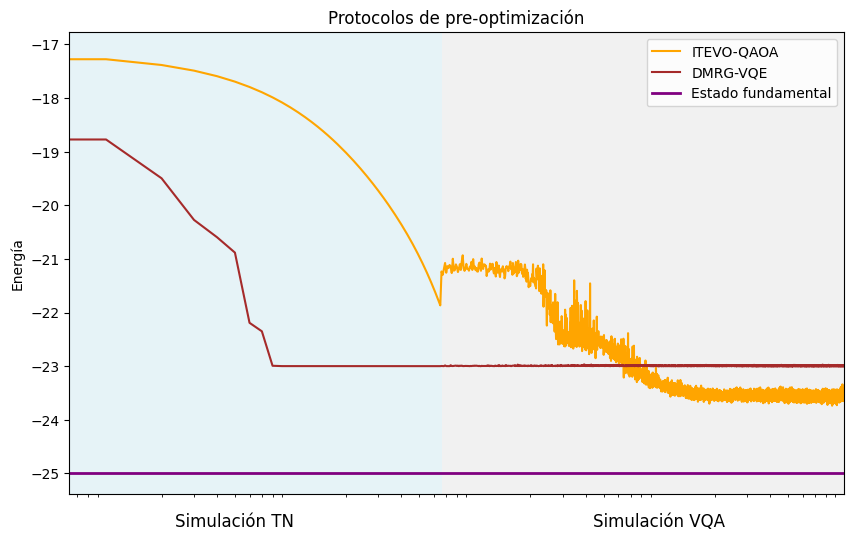
\includegraphics[scale = 0.7]{plt/06-comparativa_protocolo.png}
    \caption{comparativa de rendimiento de los protocolos de pre-optimización}
    \label{fig:comparativa_protocolo}
\end{figure}


No obstante, dado que el estado final construido por el algoritmo MPO Time Evolution es un estado de Gibbs puro de temperatura $T$, el algoritmo QAOA inicializado con dicho estado, consigue mejorar el punto de partida y mejorar al mismo tiempo el resultado conseguido por el protocolo DMRG-VQE. Además por los resultados presentados en el apartado \ref{sub_sec:result_gibbs_states}, se puede aseverar que bajo el estado de inicialización de Gibbs el algoritmo QAOA maximiza su rendimiento. \\

Otra comparativa que se podría realizar es comparar el rendimiento del algoritmo QAOA con ambos algoritmos de pre-optimización para asegurar que la diferencia de rendimiento no solo se debe por un cambio del PQC utilizado. No obstante, esta es una prueba redundante, ya que las gráficas presentadas en el apartado \ref{sub_sec:result_gibbs_states} muestran que los estados de Gibbs maximizan el rendimiento contra cualquier otro estado que esté lejos del limite de Boltzmann. El estado solución que genera el algoritmo DMRG es un estado que solo trata de minimizar $\braket{H}$ sin atender al grado de entropía del estado, por lo tanto, de forma usual el algoritmo DMRG arrojará estados solución que se encuentren alejados del limite de Boltzmann.

\newpage

Una última comparativa que es importante realizar es comparar la diferencia de rendimiento del algoritmo VQA, en este caso el algoritmo QAOA con y sin el uso del protocolo de pre-optimización. Es decir, comparar la ventaja que se obtiene cuando se utiliza un QAOA que no ha utilizado la pre-optimización con otro que si se ha servido de ello. En la Figura \ref{fig:itevo_qaoa} se compara cual es el rendimiento del algoritmo QAOA cuando trata de resolver un problema especifico de Max Cut de $N=6$ con un QAOA de $p=8$ capas.


\begin{figure}[!h]
    \centering
    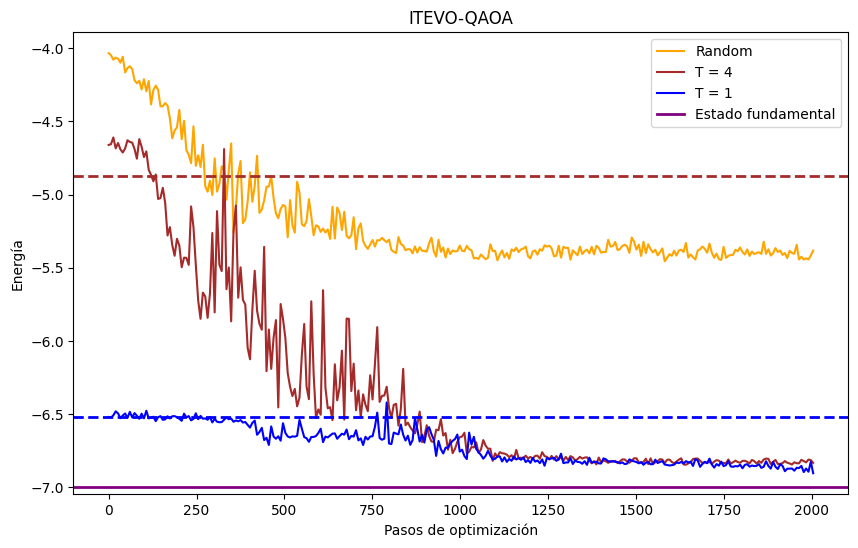
\includegraphics[scale = 0.7]{plt/06-itevo_qaoa.png}
    \caption{comparativa de rendimiento entre QAOA e ITEVO-QAOA}
    \label{fig:itevo_qaoa}
\end{figure}

Tal y como puede verse en la Figura \ref{fig:itevo_qaoa}, cuando el QAOA se inicializa con un estado inicial Hadamard, un estado de Gibbs de temperatura infinita, el algoritmo QAOA parte de un estado enérgicamente alto y se queda atrapado en mínimos locales que son sub-óptimos. Sin embargo, si se inicializa el algoritmo QAOA con estados de Gibbs de menor temperatura, el algoritmo QAOA parte de posiciones enérgicamente mas favorables, lo que le da mayor capacidad de encontrar el mínimo global. Las lineas discontinuas de la Figura \ref{fig:itevo_qaoa} hace referencia a la energía final del estado generado por el algoritmo MPO Time Evolution, para cada una de las temperaturas correspondientes.
\chapter{Conclusiones y trabajo futuro}

En este capítulo se recogen las conclusiones obtenidas después de presentar los resultados mostrados en el capítulo \ref{chapter:results} de \textit{resultados}. Además las conclusiones presentadas se ponen en relación con los objetivos e hipótesis planteadas en el capítulo \ref{chapter:goals} de \textit{objetivos}. Posteriormente se plantean posibles lineas de trabajo para continuar con el proyecto iniciado en este documento.

\section{Conclusiones}

\begin{itemize}

\item Con el desarrollo de este trabajo se ha comprendido el estado de la técnica de las estrategias que combinan algoritmos de tensor networks y algoritmos cuánticos variacionales.

\item Se ha presentado un nuevo protocolo de pre-optimización, el cual supera a su antecesor. El nuevo protocolo impide caer en estados producto de la base computacional, los cuales representan mínimos locales, evitando posteriormente, que el VQA se quede atrapado. Se sustituyen las puertas cuánticas $SU(4)$ genéricas que deben optimizarse por capas de operadores del algoritmo QAOA, aligerando enormemente el numero de parámetros a optimizar.

\item Se comprueba, a traves de simulaciones numéricas, que la magnitud entropía juega un papel fundamental en el rendimiento de los algoritmos cuánticos variacionales.

\item Los resultados expuestos sobre como los estados de Gibbs puros maximizan el rendimiento del algoritmo QAOA son bastante solidos. Se han presentado resultados en un rango amplio de tamaños, usando un problema como el Max Cut, que es NP duro.

\item Se amplia el conocimiento sobre el algoritmo QAOA. Dentro del estado de la técnica no aparecen los estados de Gibbs, excluyendo el estado Hadamard, como aquellos estados que maximizan el rendimiento del algoritmo. 

\item La pre-optimización permite reducir el uso intensivo que los VQA's hacen de los ordenadores cuánticos. Es una vía que permite que la computación cuántica tenga antes un impacto industrial relevante.

\item El protocolo de pre-optimización ITEVO-QAOA hace uso de técnicas de tensor networks para la construcción de los estados de Gibbs puros, sin embargo, cualquier otro método que permita la construcción de los estados de Gibbs que pueda ser expresado en un PQC es valido para sustituir al algoritmo MPO Time Evolution.

\end{itemize}

\section{Trabajo futuro}

Presentamos las posibles lineas de trabajo en las cuales se puede utilizar la metodología desarrollada y los resultados expuestos en el presente documento.

\begin{itemize}
    
\item Establecer una relación analítica entre los estados de Gibbs puros y el campo de energías sobre el que busca la solución un algoritmo de tipo VQA.

\item Utilizar los estados de Gibbs puros en otros algoritmos cuánticos no variacionales como el algoritmo LR-QAOA \citep{montañez}.

\item Estudio de la entropía de coherencia como métrica relevante dentro de los algoritmos cuánticos de optimización.
    
\end{itemize}


\section{Agradecimientos}

Quiero empezar las palabras de agradecimiento, citando a los tutores \textit{Dr. Arnau Riera} y \textit{Dr. Francisco Costa} que han hecho posible la realización del trabajo de fin de máster que se recoge en este documento. Por otro lado, me gustaría nombrar a  \textbf{Qilimanjaro Quantum Tech} como la empresa que me ha permitido llevar a cabo este proyecto y muy en especial a personas como Jordi, Josep, Pau, Elisabeth y muchas otras personas de Qilimanjaro que han ayudado a que este trabajo tenga la calidad que posee.
\begin{thebibliography}{a}

%1
\bibitem[Ahlander, 2002]{ahlander}
Ahlander, K. (2002) Einstein summation for multidimensional arrays.
\url{https://www.sciencedirect.com/science/article/pii/S0898122102002109}

%2
\bibitem[Amaro, 2022]{amaro}
Amaro, D., Modica, C., Rosenkranz, M., Fiorentini, M., Benedetti, M., Lubasch, M. (2022). Filtering variational quantum algorithms for combinatorial optimization. Physical Review A, 105(1), 012405. \url{https://arxiv.org/abs/2106.10055}

%3
\bibitem[Benioff, 1980]{benioff}
Benioff, P. (1980). The computer as a physical system: A microscopic quantum mechanical Hamiltonian model of computers as represented by Turing machines. Journal of Statistical Physics, 22(5), 563-591. \url{https://doi.org/10.1007/bf01011339}

%4
\bibitem[Bharti, 2021]{bharti}
Bharti, K., Cervera-Lierta, A., Kyaw, T. H., Haug, T., Alperin-Lea, S., Anand, A., Degroote, M., Heimonen, H., Kottmann, J. S., Menke, T., Mok, W.-K., Sim, S., Kwek, L.-C., Aspuru-Guzik, A. (2021). Noisy intermediate-scale quantum (NISQ) algorithms.
\url{https://arxiv.org/abs/2101.08448}

%5
\bibitem[Casazza, 2016]{casazza}
Casazza, P. G., Lynch, R. G. (2016). A brief introduction to Hilbert space frame theory and its applications.
\url{https://arxiv.org/abs/1509.07347}

%6
\bibitem[Cenedese, 2023]{cenedese}
Cenedese, G., Bondani, M., Rosa, D., Benenti, G. (2023). Generation of pseudo-random quantum states on actual quantum processors.
\url{https://www.mdpi.com/1099-4300/25/4/607}

%7
\bibitem[Cerezo, 2021]{cerezo}
Cerezo, M., Arrasmith, A., Babbush, R., Benjamin, S. C., Endo, S., Fujii, K., McClean, J. R., Mitarai, K., Yuan, X., Cincio, L., Coles, P. J. (2021). Variational quantum algorithms.
\url{https://arxiv.org/abs/2012.09265}

%8
\bibitem[Chen, 2023]{chen}
Chen, H., Barthel, T. (2023). Machine learning with tree tensor networks, CP rank constraints, and tensor dropout. Departamento de Física, ETH Zurich, Zurich, Suiza; Departamento de Física, Universidad de Duke, Durham, NC, EE.UU.; Duke Quantum Center, Universidad de Duke, Durham, NC, EE.UU.
\url{https://arxiv.org/abs/2305.19440}

%9
\bibitem[Cohen, 2019]{cohen}
Cohen-Tannoudji, C., Diu, B., Laloë, F. (2019). Quantum mechanics (Vols. I-III, 2nd ed.). Public Domain Mark 1.0 Creative Commons License.
\url{https://archive.org/details/cohen-tannoudji-diu-and-laloe-quantum-mechanics-vol.-i-ii-and-iii-2nd-ed./page/428/mode/2up}

%10
\bibitem[Dborin, 2021]{dborin}
Dborin, J., Barratt, F., Wimalaweera, V., Wright, L., Green, A. G. (2021). Matrix product state pre-training for quantum machine learning. London Centre for Nanotechnology, University College London.
\url{https://arxiv.org/abs/2106.05742}

%11
\bibitem[Deutsch, 1992]{deutsch}
Deutsch, D., Jozsa, R. (1992). Rapid solution of problems by quantum computation. Proceedings of the Royal Society of London. Series A: Mathematical and Physical Sciences, 439(1907), 553-558.
\url{https://www.isical.ac.in/~rcbose/internship/lectures2016/rt08deutschjozsa.pdf}

%12
\bibitem[Dirac, 1939]{dirac1939}
Dirac, P. A. M. (1939). A new notation for quantum mechanics. Proceedings of the Cambridge Philosophical Society, 35(4), 416-418. \url{https://www.ifsc.usp.br/~lattice/wp-content/uploads/2014/02/Dirac_notation.pdf}

%13
\bibitem[DiVincenzo, 1997]{diVincenzo}
DiVincenzo, D. P. (1997). Quantum gates and circuits. IBM Research Division, Thomas J. Watson Research Center, Yorktown Heights, NY, USA.
\url{https://arxiv.org/abs/quant-ph/9705009}

%14
\bibitem[Farhi, 2014]{farhi}
Farhi, E., Goldstone, J. (2014). A Quantum Approximate Optimization Algorithm. \url{https://arxiv.org/abs/1411.4028}

%15
\bibitem[Fernández, 2023]{fernandez}
Fernández, F. M. (2023). On the Rayleigh-Ritz variational method.
\url{https://arxiv.org/abs/2206.05122}

%16
\bibitem[Feynman, 1982]{richard}
Feynman, R. P. (1982). Simulating physics with computers. International Journal of Theoretical Physics, 21(6-7), 467-488. \url{https://doi.org/10.1007/bf02650179}

%17
\bibitem[Fröwis, 2018]{fröwis}
Fröwis, F., Nebendahl, V., Dür, W. (2018). Tensor operators: Constructions and applications for long-range interaction systems. Institut für Theoretische Physik, Universität Innsbruck.
\url{https://arxiv.org/abs/1003.1047}

%18
\bibitem[Glover, 2023]{glover}
Glover, F., Kochenberger, G., Du, Y. (2023). Quantum Bridge Analytics I: A tutorial on formulating and using QUBO models.
\url{https://wigner.hu/~koniorczykmatyas/qubo/literature/1811.11538.pdf}

%19
\bibitem[González, 2021]{bermejo} 
González Bermejo, S., Alonso-Linaje, G., Atchade-Adelomou, P. (2021). GPS: A new TSP formulation for its generalizations type QUBO. Journal of Optimization Theory and Applications, 189(1), 203-227.
\url{https://arxiv.org/abs/2110.12158}

%20
\bibitem[Heal, 2022]{heal} 
Heal, M., Dashtipour, K., Gogate, M. (2022). Formulations and algorithms to find maximal and maximum independent sets of graphs. Journal of Graph Theory.
\url{https://american-cse.org/csci2022-ieee/pdfs/CSCI2022-2lPzsUSRQukMlxf8K2x89I/202800a517/202800a517.pdf}

%21
\bibitem[Heusler, 2020]{bloch}
Heusler, S., Schlummer, P., \& Ubben, M. S. (2020). A knot theoretic extension of the Bloch sphere representation for qubits in Hilbert space and its application to contextuality and many-worlds theories. Symmetry, 12(7), 1135. \url{https://doi.org/10.3390/sym12071135}

%22
\bibitem[Hoerl, 2021]{hoerl}
Hoerl, R., Jensen, W. (2021). Understanding and addressing complexity in problem solving. Quality Engineering, 33(1), 1-15.
\url{https://www.researchgate.net/publication/354042853_Understanding_and_addressing_complexity_in_problem_solving}

%23
\bibitem[Huggins, 2018]{huggins}
Huggins, W., Patil, P., Mitchell, B., Whaley, K. B., Stoudenmire, E. M. (2018). Towards quantum machine learning with tensor networks. University of California Berkeley.
\url{https://arxiv.org/abs/1803.11537}

%24
\bibitem[Jack , 2020]{jack}
Jack, PennyLane. (s.f.). Quantum Machine Learning Demos: Tutorial on QAOA (Quantum Approximate Optimization Algorithm) Introduction. Recuperado de \url{https://pennylane.ai/qml/demos/tutorial_qaoa_intro/}

%25
\bibitem[Li, 2021]{li}
Li, J. (2021). A brief overview of graph theory: Erdos-Renyi random graph model and small world phenomenon.
\url{https://math.uchicago.edu/~may/REU2021/REUPapers/Li,Jiatong(Logen).pdf}

%26
\bibitem[Lin, 2022]{lin}
Lin, S. F., Sussman, S., Duckering, C., Mundada, P. S., Baker, J. M., Kumar, R. S., Houck, A. A., Chong, F. T. (2022). Let each quantum bit choose its basis gates. 
\url{https://arxiv.org/abs/2208.13380}

%27
\bibitem[Lucas, 2014]{lucas}
Lucas, A. (2014). Ising formulations of many NP problems. Departamento de Física, Universidad de Harvard, Cambridge, MA, USA 02138.
\url{https://arxiv.org/abs/1302.5843}

%28
\bibitem[Luis, 2023]{luis}
Luis-Hita, J., Díez-Valle, P., Hernández-Santana, S., Martínez-García, F., Díaz-Fernández, Á., Andrés, E., García-Ripoll, J. J., Sánchez-Martínez, E., Porras, D. (2023)
\url{https://arxiv.org/abs/2302.04196}

%29
\bibitem[McClean, 2018]{mcClean}
McClean, J. R., Boixo, S., Smelyanskiy, V. N., Babbush, R., Neven, H. (2018). Barren plateaus in quantum neural network training landscapes. Google Inc..
\url{https://arxiv.org/abs/1803.11173}

%30
\bibitem[Montañez, 2023]{montañez23}
Montañez-Barrera, J. A., Willsch, D., Maldonado-Romo, A., Michielsen, K. (2023). Unbalanced penalization: A new approach to encode inequality constraints of combinatorial problems for quantum optimization algorithms.
\url{https://arxiv.org/abs/2211.13914}

%31
\bibitem[Montañez, 2024]{montañez}
Montañez-Barrera, J. A.,  Michielsen, K. (2024). Towards a universal QAOA protocol: Evidence of a scaling advantage in solving some combinatorial optimization problems. Jülich Supercomputing Centre, Institute for Advanced Simulation, Forschungszentrum Jülich, Jülich, Germany; AIDAS, Jülich, Germany; RWTH Aachen University, Aachen, Germany.
\url{https://arxiv.org/abs/2405.09169}

%32
\bibitem[Mori, 2018]{mori}
Mori, T., Ikeda, T. N., Kaminishi, E., Ueda, M. (2018). Thermalization and prethermalization in isolated quantum systems: A theoretical overview. Department of Physics, Graduate School of Science, The University of Tokyo.
\url{https://arxiv.org/abs/1712.08790}

%33
\bibitem[Orús, 2014]{orus}
Orús, R. (2014). A Practical Introduction to Tensor Networks: Matrix Product States and Projected Entangled Pair States. Institute of Physics, Johannes Gutenberg University, Mainz, Germany.
\url{https://arxiv.org/abs/1306.2164}

%34
\bibitem[PennyLane, 2019]{pn}
PennyLane. (n.d.). QAOA for MaxCut. Recuperado de
\url{https://pennylane.ai/qml/demos/tutorial_qaoa_maxcut/}

%35
\bibitem[Peruzzo, 2013]{peruzzo}
Peruzzo, A., McClean, J., Shadbolt, P., Yung, M.-H., Zhou, X.-Q., Love, P. J., Aspuru-Guzik, A., O’Brien, J. L. (2013). A variational eigenvalue solver on a quantum processor. \url{https://arxiv.org/abs/1304.3061}

%36
\bibitem[Polkovnikov, 2010]{polkovnikov}
Polkovnikov, A. (2010). Microscopic diagonal entropy and its connection to basic thermodynamic relations. Department of Physics, Boston University.
\url{https://arxiv.org/abs/0806.2862}

%37
\bibitem[Preskill, 2018]{preskill}
Preskill, J. (2018). Quantum computing in the NISQ era and beyond.
\url{https://arxiv.org/abs/1801.00862}

%38
\bibitem[Ran, 2020]{ran}
Ran, S.-J. (2020). Encoding of matrix product states into quantum circuits of one- and two-qubit gates. Department of Physics, Capital Normal University.
\url{https://arxiv.org/abs/1908.07958}

%39
\bibitem[Riera, 2018]{riera}
Riera, A., Bera, M. N., Lewenstein, M., Khanian, Z. B., Winter, A. (2018). Thermodynamics as a consequence of information conservation. ICFO – Institut de Ciencies Fotoniques, The Barcelona Institute of Science and Technology.
\url{https://arxiv.org/abs/1707.01750}

%40
\bibitem[Rudolph, 2022]{rudolph}
Rudolph, M. S., Chen, J., Miller, J., Acharya, A.,  Perdomo-Ortiz, A. (2022). Decomposition of matrix product states into shallow quantum circuits. Zapata Computing Canada Inc.
\url{https://arxiv.org/abs/2209.00595}

%41
\bibitem[Rudolph, 2023]{manuel}
Rudolph, M. S., Miller, J., Motlagh, D., Chen, J., Acharya, A., Perdomo-Ortiz, A. (2023). Synergy between quantum circuits and tensor networks: Short-cutting the race to practical quantum advantage. Zapata Computing.
\url{https://arxiv.org/abs/2208.13673}

%42
\bibitem[Schollwöck, 2011]{schollwöck}
Schollwöck, U. (2011). The density-matrix renormalization group in the age of matrix product states. Department of Physics, Arnold Sommerfeld Center for Theoretical Physics and Center for NanoScience, University of Munich.
\url{https://arxiv.org/abs/1008.3477}

%43
\bibitem[Shannon, 1948]{Shannon1948} 
Shannon, C. E. (1948). A Mathematical Theory of Communication. The Bell System Technical Journal, 27, 379–423, 623–656. (Reprinted with corrections from July, October, 1948).
\url{https://people.math.harvard.edu/~ctm/home/text/others/shannon/entropy/entropy.pdf}

%44
\bibitem[Shaydulin, 2024]{shaydulin}
Shaydulin, R., He, Z., Chakrabarti, S., Herman, D., Li, C., Sun, Y., Pistoia, M. (2024). Alignment between initial state and mixer improves QAOA performance for constrained optimization. Global Technology Applied Research, JPMorgan Chase, New York, NY.
\url{https://arxiv.org/abs/2305.03857}

%45
\bibitem[Shirakawa, 2021]{shirakawa}
Shirakawa, T., Ueda, H.,  Yunoki, S. (2021). Automatic quantum circuit encoding of a given arbitrary quantum state. Computational Materials Science Research Team, RIKEN Center for Computational Science (R-CCS).
\url{https://arxiv.org/abs/2112.14524}

\newpage

%46
\bibitem[Shor, 1994]{shor}
Shor, P. W. (1994). Polynomial-time algorithms for prime factorization and discrete logarithms on a quantum computer. Proceedings of the 35th Annual Symposium on Foundations of Computer Science, 124-134.
\url{https://arxiv.org/abs/quant-ph/9508027}

%47
\bibitem[Tensor Network, n.d.]{tn}
Tensor Network. (n.d.). Matrix product operator (MPO). Recuperado de
\url{https://tensornetwork.org/mpo/}

%48
\bibitem[Tucci, 2008]{tucci}
Tucci, R. R. (2008). An introduction to Cartan’s KAK decomposition for QC programmers. P.O. Box 226, Bedford, MA.
\url{https://arxiv.org/abs/quant-ph/0507171}

%49
\bibitem[Xi, 2015]{xi}
Xi, Z., Li, Y., Fan, H. (2015 ). Quantum coherence and correlations in quantum systems.
\url{https://arxiv.org/abs/1408.3194}

%50
\bibitem[Yang, 2020]{yang} 
Yang, Q., Li, Y., Huang, P. (2020). A novel formulation of the max-cut problem and related algorithm. Journal of Combinatorial Optimization.
\url{https://www.sciencedirect.com/science/article/abs/pii/S0096300319309622}

%51
\bibitem[Zaletel, 2014]{zaletel}
Zaletel, M. P., Mong, R. S. K., Karrasch, C., Moore, J. E., Pollmann, F. (2014). Time-evolving a matrix product state with long-ranged interactions. Physical Review B, 90(4), Article 045113.
\url{https://arxiv.org/abs/1407.1832}

%52
\bibitem[Zhu, 2022]{zhu}
Zhu, L., Tang, H. L., Barron, G. S., Calderon-Vargas, F. A., Mayhall, N. J., Barnes, E., Economou, S. E. (2022). An Adaptive Quantum Approximate Optimization Algorithm for Solving Combinatorial Problems on a Quantum Computer. Physical Review A, 106(1), 012403. \url{https://arxiv.org/abs/2005.10258}

\end{thebibliography}
\appendix
\chapter{Apéndices}

\section{Resultados algoritmo DMRG}
\label{apendix:dmrg}

En este apéndice presentamos resultados numéricos del funcionamiento del algoritmo DMRG. El problema a resolver por el algoritmo DMRG es el problema Max Cut, presentado en el apartado \ref{sub:problem_target}. La calidad del resultado obtenido por el algoritmo DMRG depende del numero de pasos de optimización realizados y de la dimensión interna considerada para mapear el Hamiltoniano en un MPO así como la dimensión interna máxima permitida para representar el estado solución en un MPS. Tal y como puede verse en la Figura \ref{fig:result_dmrg}, la calidad de la solución obtenida depende de la dimensión interna $\chi$ que posee tanto el MPO como el MPS que participa en el proceso de optimización.

\begin{figure}[!h]
    \centering
    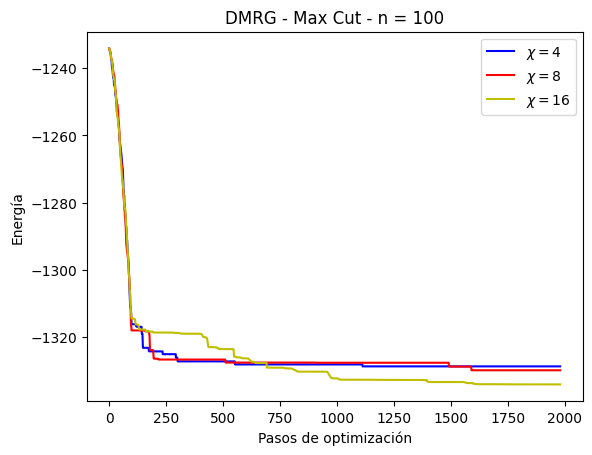
\includegraphics[scale = 0.7]{plt/a01-dmrg_max_cut_n_100.png}
    \caption{resultados DMRG problema Max Cut para 100 nodos}
    \label{fig:result_dmrg}
\end{figure}

Con pocos pasos de optimización, la calidad de la solución obtenida puede ser mejor con un $\chi$ bajo, dado que el subespacio de Hilbert en el que busca el algoritmo DMRG es menor y por lo tanto encuentra antes cual es el estado $\psi$ de ese subespacio que minimiza la energía del MPO. 

\newpage

\section{Resultados de los algoritmos de traducción}
\label{apendix:mps_to_pqc}

En este apéndice se presentan resultados orientados a mostrar las particularidades de los algoritmos de traducción de MPS a PQC.

\subsection{Traducción analítica}

El protocolo de traducción analítica permite construir cada capa de operadores unitarios de dos qubits en base a unas reglas fijas. Estas reglas permiten construir los tensores $G$ de dos qubits los cuales tienen una correspondencia directa con operadores de dos qubits, tal y como se observa en la Figura \ref{fig:mpd_to_pqc}. Las reglas las cuales permiten construir los tensores $G$ a partir de los tensores $A$ pertenecientes al MPS de $\chi =2$ vienen dado por el conjunto de expresiones \ref{eq:rules_mps_to_pqc}.

\begin{equation}
\begin{aligned}
G^{[8]} &= A^{[8]} \\
G_{00kl}^{[1]} &= A_{kl}^{[1]} \\
G_{0jkl}^{[n]} &= A_{jkl}^{[n]} \\
\sum_{kl} G^{[n]}_{i^{'} j^{'} k l} G^{[n]*}_{i j k l} &= I_{i^{'} i} I_{j^{'} j}
\end{aligned}
\label{eq:rules_mps_to_pqc}
\end{equation}

El protocolo de traducción analitico aún siendo eficiente en terminos de coste computacional, arroja resultados poco precisos cuando la dimesión $\chi$ del MPS que se desea replicar crece.


\begin{figure}[!h]
    \centering
    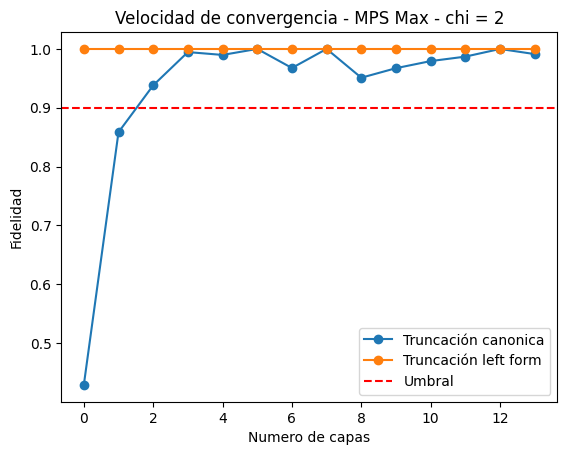
\includegraphics[scale = 0.6]{plt/a02-mps_to_pqc_a.png}
    \caption{resultados del proceso de traducción analítica de un MPS de $\chi = 2$ a PQC}
    \label{fig:r_mps_to_pqc_a}
\end{figure}

\newpage

Tal y como se puede observar en la Figura \ref{fig:r_mps_to_pqc_a}, con un MPS inicial de $\chi = 2$, existen inestabilidades numéricas asociadas a la metodología  \textit{canónica} la cual requiere de mas capas para poder replicar un MPS de $\chi = 2$, cuando idealmente solo necesita una, tal y como ocurre con el método \textit{left form}. El umbral marca la fidelidad a partir del cual podemos detener el proceso de traducción. Por otro lado, cuando se intenta traducir a un PQC, un MPS de $\chi > 2$ encontramos que las inestabilidades numéricas lo impiden, tal y como puede verse en la Figura \ref{fig:r_mps_to_pqc_a_2}.


\begin{figure}[!h]
    \centering
    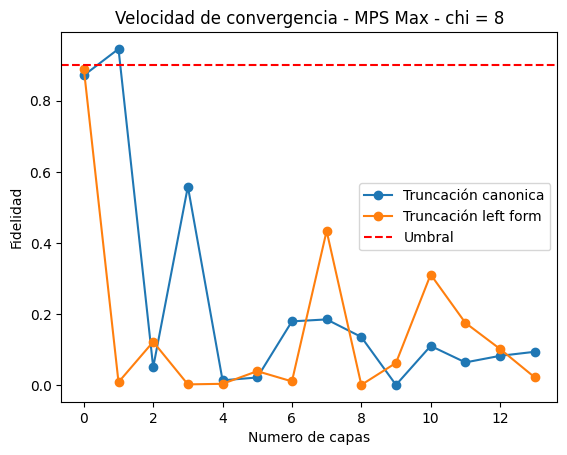
\includegraphics[scale = 0.7]{plt/a03-mps_to_pqc_a_2.png}
    \caption{resultados del proceso de traducción analítica de un MPS de $\chi = 8$ a PQC}
    \label{fig:r_mps_to_pqc_a_2}
\end{figure}

En \ref{fig:r_mps_to_pqc_a_2} se observa como mayor numero de capas no garantiza una mejora en la fidelidad conseguida entre el MPS inicial y el PQC generado.

\subsection{Traducción por optimización}

El método de traducción por optimización de MPS a PQC siendo mas costoso computacionalmente genera resultados los cuales son mas consistentes y precisos. Tal y como puede observarse en la Figura \ref{fig:r_mps_to_pqc_o} el algoritmo de traducción por optimización consigue replicar un MPS de $\chi = 64$ con tan solo 2 y 4 capas de un PQC. En general se puede replicar un MPS, si este contiene solo coeficientes reales, de $\chi = n$ con un PQC que tenga, en terminos de $\chi$, un valor menor. Cada capa de PQC, implica un aumento de \textit{x4} en el aumento de $\chi$, de tal forma que un PQC de dos capas generan un MPS de $\chi = 16$.

\newpage

\begin{figure}[!h]
    \centering
    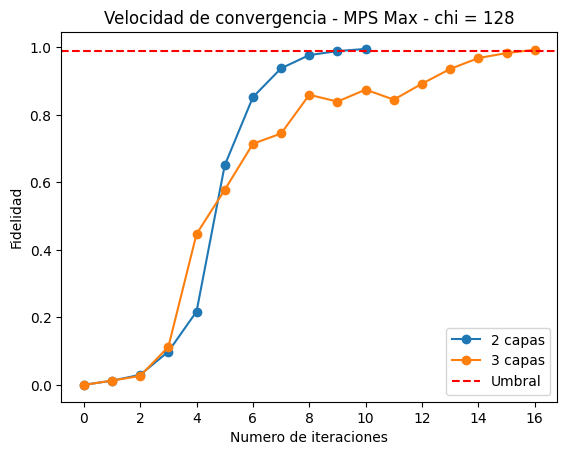
\includegraphics[scale = 0.7]{plt/a04-mps_to_pqc_o.png}
    \caption{resultados del proceso de traducción por optimización de un MPS de $\chi = 128$ a PQC}
    \label{fig:r_mps_to_pqc_o}
\end{figure}

La propiedad de replicar estados de MPS en PQC's de dimesión $\chi$ inferior es utilizada en algoritmos ciertos algoritmos de compresión.

\section{Resultados algoritmo MPO Time Evolution}
\label{apendix:mpo_time_evolution}

En este apéndice presentamos resultados numéricos del funcionamiento del algoritmo MPO Time Evolution. El MPO Time evolution es usado para implementar la evolución temporal imaginaria del sistema cuántico. El problema a resolver por el algoritmo MPO Time Evolution, al igual que el algoritmo DMRG, es el problema Max Cut, presentado en el apartado \ref{sub:problem_target}. De forma análoga al algoritmo DMRG, la calidad de la solución obtenida por el algoritmo MPO Time Evolution depende del tiempo de evolución durante el cual se hace evolucionar al sistema, así como la discretización $\delta \tau$ utilizada, y de la dimesión interna $\chi$ máxima permitida tanto para el MPS, que representa el estado cuántico, como para el MPO, que representa el Hamiltoniano. En la Figura \ref{fig:result_tevo} se puede observar como la calidad de la solución encontrada está influida fuertemente por la discretización del tiempo usada. Es importante recordar que el error asociado al MPO Time evolution es del orden de $(\delta \tau)^2$, lo cual limita no solo la calidad de la solución encontrada si no también la calidad del estado de Gibbs puro construido.

\newpage

\begin{figure}[!h]
    \centering
    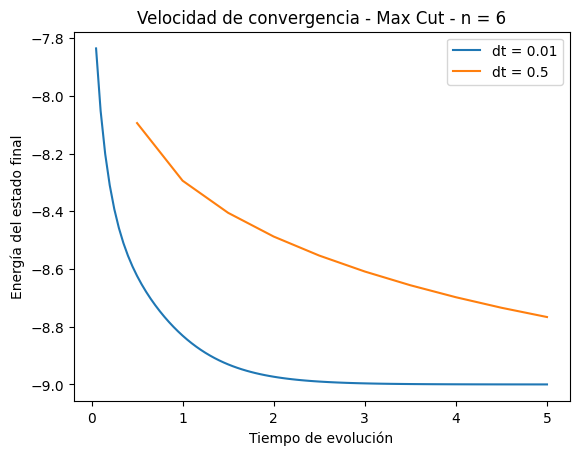
\includegraphics[scale = 0.7]{plt/a05-tevo_max_cut_n_6.png}
    \caption{resultados MPO Time Evolution para un Max Cut de 6 nodos}
    \label{fig:result_tevo}
\end{figure}

Es importante demostrar que los estados construidos son realmente estados de Gibbs de la temperatura esperada. Para comprobar que los estados generados son realmente estados de Gibbs podemos utilizar el hecho de conocer cual es la distribución de probabilidad esperada. Se sabe que los coeficientes de un estado de Gibbs puro viene dado por la expresión \ref{eq:coeficient_gibbs}.

\begin{equation}
c_{i} = \frac{e^{- \frac{E_{i}}{T}}}{Q}
\label{eq:coeficient_gibbs}
\end{equation}

Donde el factor $Q$ representa la constante de normalización del estado, $T$ la temperatura asociada y $E_{i}$ la energía asociado al autoestado del Hamiltoniano $\ket{i}$. Tomando el logaritmo en base $e$ de la expresión \ref{eq:coeficient_gibbs} obtenemos la expresión \ref{eq:coeficient_gibbs_log}.

\begin{equation}
\log(c_{i}) = \frac{- E_{i}}{T} - \log(Q)
\label{eq:coeficient_gibbs_log}
\end{equation}

Dada la forma de la expresión \ref{eq:coeficient_gibbs_log}, si se representa la energía como valor $x$ de una función y el logaritmo de $c_{i}$ como el valor $y$ de la función, debemos esperar que la función será una recta de pendiente $-\frac{1}{T}$. Esto es lo que se ha representado en la Figura \ref{fig:result_gibbs_pb}, para comprobar que el algoritmo MPO Time Evolution implementa correctamente los estados de Gibbs puros.

\newpage

\begin{figure}[!h]
    \centering
    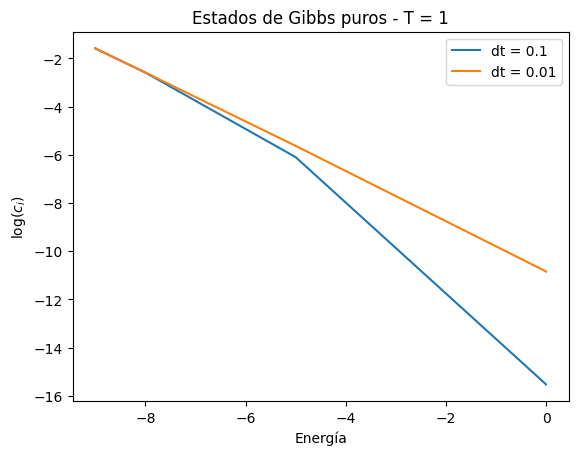
\includegraphics[scale = 0.7]{plt/a06-gibbs_state_pb.png}
    \caption{distribución de probabilidad para un estado de Gibbs puro de $T=1$}
    \label{fig:result_gibbs_pb}
\end{figure}

Para la Figura \ref{fig:result_gibbs_pb} se puede observar como la pendiente de la recta posee valor $p=-1$, que es la temperatura esperada del estado de Gibbs.

\section{Análisis del campo de energías}
\label{apendix:energy_landscape}

Una forma de intentar descubrir por que los estados de Gibbs maximizan el rendimiento del algoritmo QAOA es mediante un análisis del campo de energías en el cual algoritmo QAOA trata de encontrar el mínimo global. El algoritmo QAOA formando por una sola capa, contiene dos operadores parametrizados, cada uno de ellos con ángulo a optimizar, tal y como se ve en la expresión \ref{eq:pqc_qaoa_one_layer}.


\begin{equation}
    U(\gamma,\beta)= e^{-i \gamma H_C} e^{- i \beta H_M}
    \label{eq:pqc_qaoa_one_layer}
\end{equation}

Dado el QAOA formado por una sola capa, a traves del operador de la expresión \ref{eq:pqc_qaoa_one_layer}, que posee solo dos parámetros, podemos visualizar directamente el campo de energías. En la Figura \ref{fig:landscape_energy} se muestra cual es el campo de energías que genera el algoritmo QAOA de una sola capa para un problema concreto de Max Cut de $N=7$. El estado de Gibbs y el estado de pseudoGibbs poseen la misma energía pero el estado de pseudoGibbs contiene ligeramente menor entropía. 

\newpage

Los ejes $x$ e $y$ de ambos gráficos hacen referencia al valor que toman los parámetros $\alpha$ y $\beta$. El código de colores hace referencia al valor esperado energía que se obtiene cuando se ejecuta el QAOA con los valores de $\alpha$ y $\beta$ correspondientes.

\begin{figure}[!h]
    \centering
    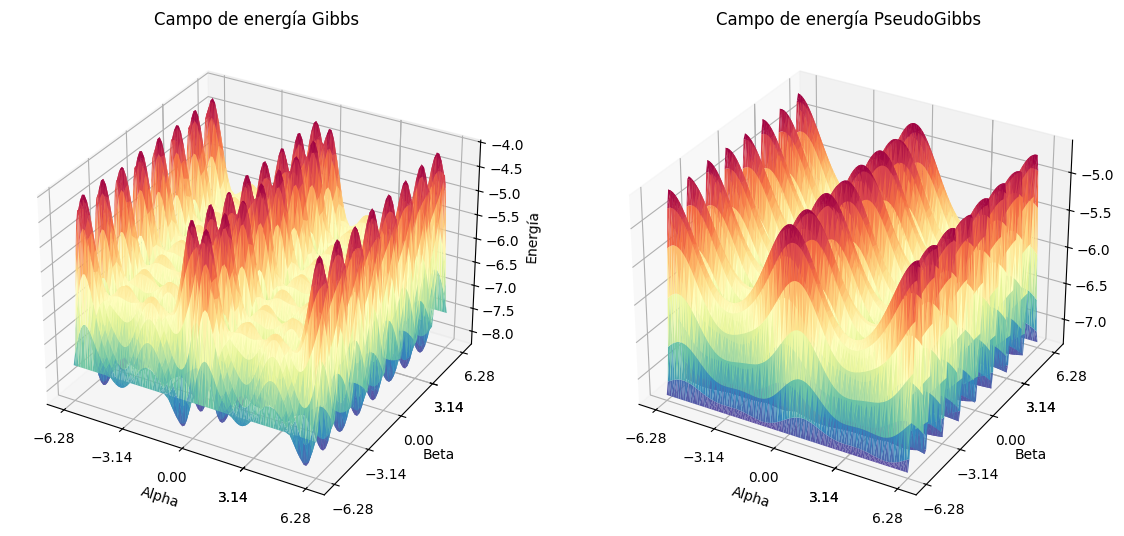
\includegraphics[scale = 0.55]{plt/a07-energy_landscape.png}
    \caption{campos de energías para estados de Gibbs y de pseudoGibbs de igual energía}
    \label{fig:landscape_energy}
\end{figure}

En la Figura \ref{fig:landscape_energy} puede observarse como el estado de Gibbs mejora la expresividad del circuito QAOA permitiendo encontrar mínimos globales mas profundos, a diferencia del circuito QAOA inicializado con el estado de pseudoGibbs. La mejorar del rendimiento del algoritmo QAOA cuando se utilizan estados de Gibbs puros como estados de inicialización puede deberse en parte al hecho de que se mejora la expresividad del circuito QAOA.

\end{document}
